\documentclass[10pt,conference,compsocconf]{IEEEtran}
\usepackage[T1]{fontenc}
\font\chinesefont="Songti SC" at 10pt
\usepackage{cite}
\usepackage{amsmath,amssymb}
\usepackage{graphicx,booktabs,array,tabularx}
\usepackage{float,algpseudocode}
\floatstyle{ruled}
\newfloat{algorithm}{tbp}{loa}
\floatname{algorithm}{Algorithm}
\usepackage{flushend}
\usepackage{tikz}
\usetikzlibrary{arrows.meta,positioning}
\usepackage{xcolor}
\usepackage{xurl}
\definecolor{citationblue}{RGB}{0,70,180}
% Light-red marks text revised in the latest pass; set to black to hide.
\definecolor{revisedred}{RGB}{226,86,86}
\newcommand{\rev}[1]{{\color{revisedred}#1}}
\newenvironment{revised}{\color{revisedred}}{}
% Light orange marks content waiting for the Laya-only MACRON run.
\definecolor{pendingorange}{RGB}{238,146,40}
\newcommand{\pend}[1]{{\color{pendingorange}#1}}
\newenvironment{pending}{\color{pendingorange}}{}
\usepackage[colorlinks=true,citecolor=citationblue,linkcolor=black,urlcolor=black]{hyperref}
\hypersetup{pdftitle={Boyun: Multi-Agent Simulation for Financial and Economic Decisions},pdfauthor={Cherry Q},pdfsubject={Financial and economic simulation with explicit actor incentives}}
\setlength{\emergencystretch}{1.5em}
\newcolumntype{Y}{>{\raggedright\arraybackslash}X}
\newtheorem{proposition}{Proposition}
\renewcommand{\thesection}{\Roman{section}}
\definecolor{ink}{HTML}{17352F}
\definecolor{teal}{HTML}{267267}
\definecolor{wash}{HTML}{EEF5F2}
\tikzset{box/.style={draw=teal!70,rounded corners=2pt,fill=wash,align=center,font=\small,minimum height=0.95cm,text width=4.3cm,inner sep=5pt},arr/.style={-{Latex[length=2mm]},thick,draw=teal}}
\title{\textit{Boyun}: Multi-Agent Simulation\\for Financial and Economic Decisions\\\large Draft}
\author{\IEEEauthorblockN{Cherry Q}}
% Keep IEEE heading spacing; emphasize both labels and titles in the draft.
\makeatletter
\renewcommand{\section}{\@startsection{section}{1}{\z@}{1.5ex plus 1.5ex minus 0.5ex}%
{0.7ex plus 1ex minus 0ex}{\normalfont\normalsize\centering\itshape}}
\renewcommand{\subsection}{\@startsection{subsection}{2}{\z@}{1.5ex plus 1.5ex minus 0.5ex}%
{0.7ex plus .5ex minus 0ex}{\normalfont\normalsize\itshape}}
\renewcommand{\subsubsection}{\@startsection{subsubsection}{3}{\parindent}{0ex plus 0.1ex minus 0.1ex}%
{0ex}{\normalfont\normalsize\itshape}}
\makeatother
\begin{document}
\raggedbottom
\maketitle
% Abstract revised in the working draft.
\begin{abstract}
Financial and economic decisions are shaped by actors with different goals,
resources, and information, whose actions influence one another over time.
Understanding these decisions requires explicit models of strategic choices,
information exchange, and uncertainty. We present \textit{Boyun}, a
\rev{self-hosted, locally executed} multi-agent simulation framework for
exploring such decisions in specified worlds. Its construction draws on
\textit{game theory} to define \rev{actors, preference weights,} feasible
actions, and consequences; \textit{directed information graphs} to represent
who receives \rev{messages}; and \textit{probability and statistics} to examine
declared uncertainty and evaluate probabilistic claims. \rev{Actors} receive
restricted observations, and \rev{a local actor decision model}, \textit{Laya},
returns structured choices and option scores \rev{on the user's own hardware}.
An execution engine applies the specified rules \rev{across strategic, market,
and lending ledgers} and records state transitions. The resulting record
supports inspection of observations, choices, and numerical consequences, and
allows execution to be replayed from saved decisions without repeating
inference. A local agent interface supports caller-authored worlds and offline
experiments, and an optional blockchain commitment supports later verification
of artifact integrity. Six synthetic experiments reproduce hand-calculated
game, Bayesian, scoring, and accounting results and isolate individual
mechanisms. \rev{Running locally with \textit{Laya} at zero API fee, a
fourteen-day, sixteen-actor token-launch case completes all 24 policy paths
with settled trades, recorded rejections, matched branch comparisons, and exact
replay, while} a comparison with the original \textit{MiroFish} on the same
brief shows that the two systems are complementary: one produces richer social
discourse, the other settled financial consequences. \rev{In addition, a
ninety-day collateralized lending case across four worlds separates mechanical
conclusions fixed by ledger rules from behavioral ones sensitive to uncalibrated
actor scores.} These results do not establish human behavioral fidelity, market
forecasting accuracy, or improved decision quality; these claims require
further empirical and comparative evaluation.
\end{abstract}
\begin{IEEEkeywords}
Game theory, multi-agent simulation, agent-based modeling, social graphs, probability, statistical evaluation, scenario analysis.
\end{IEEEkeywords}
\begin{figure*}[t]
\centering\color{revisedred}
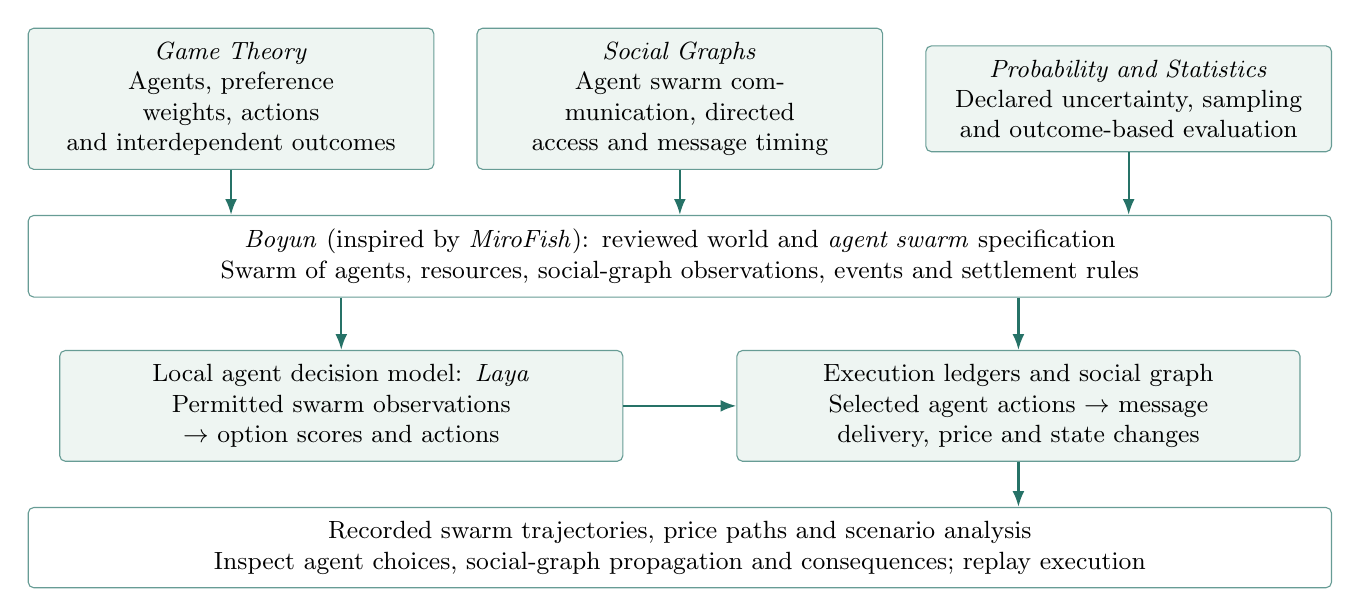
\begin{tikzpicture}[
 foundation/.style={draw=teal!70,fill=wash,rounded corners=2pt,align=center,text width=4.8cm,minimum height=1.25cm,inner sep=5pt,font=\small},
 layer/.style={draw=teal!70,fill=white,rounded corners=2pt,align=center,text width=16.2cm,minimum height=0.85cm,inner sep=5pt,font=\small},
 component/.style={draw=teal!70,fill=wash,rounded corners=2pt,align=center,text width=6.8cm,minimum height=1.1cm,inner sep=5pt,font=\small},
 connection/.style={-{Latex[length=2mm]},draw=teal,thick}]
\node[foundation] (game) at (0,0) {\textit{Game Theory}\\Agents, preference weights, actions\\and interdependent outcomes};
\node[foundation] (graph) at (5.7,0) {\textit{Social Graphs}\\Agent swarm communication, directed\\access and message timing};
\node[foundation] (prob) at (11.4,0) {\textit{Probability and Statistics}\\Declared uncertainty, sampling\\and outcome-based evaluation};
\node[layer] (world) at (5.7,-2) {\textit{Boyun} (inspired by \textit{MiroFish}): reviewed world and \textit{agent swarm} specification\\Swarm of agents, resources, social-graph observations, events and settlement rules};
\draw[connection] (game.south)--(game.south |- world.north);
\draw[connection] (graph.south)--(world.north);
\draw[connection] (prob.south)--(prob.south |- world.north);
\node[component] (laya) at (1.4,-3.9) {Local agent decision model: \textit{Laya}\\Permitted swarm observations $\rightarrow$ option scores and actions};
\node[component] (engine) at (10,-3.9) {Execution ledgers and social graph\\Selected agent actions $\rightarrow$ message delivery, price and state changes};
\draw[connection] (world.south -| laya.north)--(laya.north);
\draw[connection] (world.south -| engine.north)--(engine.north);
\draw[connection] (laya.east)--(engine.west);
\node[layer] (record) at (5.7,-5.7) {Recorded swarm trajectories, price paths and scenario analysis\\Inspect agent choices, social-graph propagation and consequences; replay execution};
\draw[connection] (engine.south)--(engine.south |- record.north);
\end{tikzpicture}
\caption{\rev{Foundations of \textit{Boyun}, inspired by \textit{MiroFish}. The
upper row identifies conceptual foundations; the lower layers show how modeled
actors operate as a \textit{swarm of agents} communicating over a \textit{social
graph} while self-hosted \textit{Laya} supplies live agent decisions locally and
deterministic ledgers apply the specified rules.} Probability and statistical tools are separate
analytical components, not automatic calibration of the agent decision model.
Probability calculations use declared inputs; neither the diagram nor replay
implies calibrated predictions or empirically validated social influence.}
\label{fig:foundations}
\end{figure*}

\section{Introduction}\label{sec:introduction}
Financial and economic decisions depend on how people and organizations
respond to one another under uncertainty. A protocol designer evaluating an
incentive must weigh its direct cost, whether partners join, and how other
actors react, since those reactions alter the choices available later.
Comparing alternatives therefore requires scenarios that make actors,
constraints, and assumed events explicit while showing how their interactions
produce different outcomes.

To that end, \textit{agent-based modeling} represents a system through
\rev{an interacting \textit{swarm of agents}---autonomous decision-makers whose
local observations and actions follow explicit interaction rules---}so its
conclusions depend on both the assumptions and their implementation
\cite{grimm2020,galan2009}. However, although language-model agents can
condition choices on context \cite{park2023,yang2025}, an expressed choice
alone does not specify its economic consequences. For example, a disclosure
decision \rev{emitted by one agent in a swarm} still requires rules defining
which \rev{connected agents receive the message over a social graph}, when they
react, and what resource or state changes follow.

Along another dimension, social-simulation frameworks examine \rev{how an
\textit{agent swarm} interacts across a shared social graph}. \textit{OASIS}
(Open Agent Social Interaction Simulations) provides one such platform, while
\textit{MiroFish} uses \rev{an agent-swarm social-simulation} workflow to
explore scenarios \cite{yang2025,mirofish}. \rev{Inspired directly by
\textit{MiroFish}'s paradigm of constructing worlds, orchestrating an
interacting swarm of agents, and synthesizing scenario reports,} \textit{Boyun}
pursues specialized financial and economic analysis, combining complementary
methods to connect strategic incentives, \rev{social-graph communication across
an agent swarm,} and numerical consequences.

\rev{Building on that \textit{MiroFish}-inspired agent-swarm foundation,} we
present \textit{Boyun} ({\chinesefont 拨云}, {\chinesefont bō yún}), a
self-hosted \rev{\textit{agent-swarm}} framework for exploring decisions
through explicit simulated worlds. Its Chinese name means ``part the clouds''
and draws on {\chinesefont 拨云见日}, in which clouds are parted to reveal the
sun. \rev{In \textit{Boyun}, market and protocol actors are modeled as
autonomous \textit{agents} that communicate with one another across a
\textit{social graph} as a \textit{swarm of agents}.} The name expresses the
aim of bringing \rev{that agent swarm}, its incentives, assumptions,
\rev{social-graph relationships}, and possible consequences into view before
action, while keeping that view conditional on the evidence and assumptions
used to construct it. Figure~\ref{fig:foundations} summarizes the foundations
and their operational roles.

First, to give this \rev{agent swarm} an executable structure, \textit{Boyun}
places \textit{game theory} at the center of world construction. \rev{Agents in
the swarm} have preference weights, resources, information, and feasible
actions, and the world's rules determine how their combined choices affect
outcomes \cite{polak2,nash1950}. This structure makes incentives, coordination,
and conflicts of interest explicit without assuming that model-selected actions
are optimal or form an equilibrium. The distinction matters whenever
\rev{agents} value different outcomes: a founder \rev{agent} may prioritize
participation, whereas a partner \rev{agent} may prioritize credibility or
retained capital. Such differences must alter feasible actions and their
consequences rather than remain descriptive labels in a persona.

On the other hand, incentives alone do not specify who knows what when \rev{inside
the swarm}. \textit{Boyun} therefore \rev{connects the \textit{swarm of agents}
through a \textit{social graph}---formalized as a \textit{directed information
graph}---that specifies which agents receive another agent's messages and how
signals propagate across the swarm}. Message availability and timing thus
become explicit parts of the world rather than hidden assumptions. Even so,
these \rev{social-graph} links describe permitted delivery rather than
empirically measured social influence, allowing an analyst to test how a
disclosure, delayed message, or restricted channel changes \rev{what each agent
in the swarm observes} without giving every \rev{agent} the author's complete
view.

Apart from strategic incentives and \rev{social-graph} communication, events
and outcomes often remain uncertain. \textit{Probability and statistics}
provide a third foundation: \textit{Bayesian} calculations update supplied
beliefs, seeded sampling explores declared alternatives, and proper scoring
rules evaluate probabilistic predictions \cite{pishronik2014,brier1950,gneiting2007}.
Nevertheless, these tools expose uncertainty only under stated assumptions;
neither repeated simulation nor model confidence establishes real-world odds.

Once those three foundations define a world, the engine must obtain \rev{choices
across the \textit{agent swarm}} while keeping local inference and recorded
execution explicit. Because unpublished launch plans, treasury limits, and risk
parameters are sensitive, \textit{Boyun} focuses on private, self-hosted
execution using an open-weight \rev{\textit{agent decision model}} that runs
locally on the user's hardware. Each \rev{agent in the swarm} receives only its
permitted \rev{social-graph and ledger} observation, and \textit{Laya}
\cite{layamodel}---the local \rev{agent} model used in the reported case
studies---returns a structured choice and normalized \textit{option scores}
over the \rev{agent's} \textit{affordable action menu}. Alternative open-weight
models are a future evaluation direction rather than a capability demonstrated
by these runs. Crucially, option scores express model-assigned weights rather
than validated real-world probabilities. Deterministic strategic, market, and
lending ledgers then settle the chosen actions, \rev{route messages across the
social graph,} enforce conservation, and save every observation and choice so
runs replay exactly without repeating inference, while leaving the model's
internal deliberation unobserved.

Moreover, self-hosted inference addresses a practical budget constraint.
\rev{Evaluating an \textit{agent swarm} across many decision points, social-graph
interactions,} and matched policy branches requires tens or hundreds of
thousands of model queries, which quickly exhaust small hosted-API budgets while
sending private scenario states off the user's machine. Running \textit{Laya}
locally eliminates per-call API fees and keeps all \rev{swarm} observations
on-device, though operational efficiency and behavioral accuracy remain separate
evaluation questions.

Given these capabilities and boundaries, the paper asks: \emph{Can a
self-hosted, explicitly specified \rev{agent-swarm} world constrain
\rev{social-graph} information, spending, and settlement while making the
effects of alternative information and interaction rules inspectable?}
Applications include capital allocation, participation incentives, disclosure
policies, and credit stress scenarios in decentralized finance. Reports connect
financial outcomes \rev{and simulated price paths} with coordination,
\rev{social-graph} message delivery, and \rev{swarm} reactions to events so
researchers, protocol designers, and risk analysts can trace how an outcome
arises under declared assumptions.

Accordingly, we evaluate \textit{Boyun} through six synthetic mechanism
experiments, a fourteen-day \rev{sixteen-agent swarm} token-launch case across
24 policy paths and a ninety-day \rev{twenty-agent swarm} collateralized lending
case across four worlds---all executed locally with \textit{Laya}---together
with a matched-brief comparison against the original \textit{MiroFish} \rev{that
inspired \textit{Boyun}'s workflow}. These tests do not establish human
behavioral fidelity, forecasting accuracy, or improved user decisions. Within
that scope, the paper makes five contributions:
\begin{enumerate}\setlength{\itemsep}{1pt}
\item an explicit specification of worlds, \rev{the \textit{swarm of agents},
and what each agent may observe over the \textit{social graph}}
(Section~\ref{sec:world-creation});
\item an execution procedure across strategic, market, and lending ledgers that
records every \rev{agent} decision and replays it exactly
(Section~\ref{sec:method-system});
\item reproducible mechanism tests with known answers
(Sections~\ref{sec:evaluation}--\ref{sec:results});
\item a matched case comparison with the original \textit{MiroFish}
(Section~\ref{sec:res-mirofish});
\item full-horizon local \textit{Laya} token-launch and lending case studies
\rev{---including simulated token-price trajectories across 24 worlds---}that
separate mechanical conclusions fixed by ledger rules from behavioral ones
sensitive to the \rev{agent} decision model (Sections~\ref{sec:res-macron}
and~\ref{sec:res-lending}).
\end{enumerate}
The following section situates these contributions within prior work.

\section{Related Work}\label{sec:related}
The Introduction linked strategic incentives, message delivery, and uncertainty
within a self-hosted simulated world. To situate that design, this section
first examines how agent-based models are specified, and then reviews
game-theoretic and financial environments, social simulation, and probabilistic
decision evaluation. Throughout, comparisons concern modeling scope and
preserved evidence rather than a performance ranking of systems.

\subsection{Agent-Based Simulation and Model Specification}
To make interacting actors a reproducible object of study, agent-based research
requires an explicit description of the environment and its rules. In
particular, the Overview, Design concepts, and Details (\textit{ODD}) protocol
standardizes descriptions of entities, initialization, schedules, inputs, and
submodels \cite{grimm2020}. Complementing specification standards,
Gal\'an et al.\ distinguish conceptual modeling assumptions from artifacts
introduced by software implementation \cite{galan2009}. Together, these works
motivate separating verification---whether code executes stated rules
accurately---from validation of whether those rules represent real markets.

Building on that distinction, \textit{Boyun} specifies actors,
resources, observation boundaries, actions, and settlement rules before a run
begins. Preserving these inputs opens assumptions to review and enables exact
replay checks. However, an explicit specification alone cannot show that
assumed incentives or actor choices are realistic, which requires examining
both the economic environment and the behavioral model.

\subsection{Game-Theoretic and Economic Environments}
On the strategic side, \textit{game theory} links actors' choices to
outcomes that depend on what others do. \textit{Nash equilibrium} provides a
classic benchmark in which no actor gains from a unilateral deviation
\cite{nash1950}, and \textit{OpenSpiel} operationalizes finite games through
explicit states, legal actions, observations, transitions, and returns
\cite{lanctot2019}. \textit{Boyun} adopts explicit game specification to
construct decision worlds; by contrast, it neither incorporates
\textit{OpenSpiel}'s equilibrium solvers nor assumes that its actor decision
model plays an equilibrium.

Beyond abstract games, economic simulation environments enforce
incentives through allocation and accounting rules. For instance, the
\textit{AI Economist} couples economic agents with a tax-policy planner,
separating individual utility from a designer's objective \cite{zheng2020},
while \textit{EconAgent} places language-model agents inside numerical
macroeconomic rules for labor and consumption \cite{li2024econagent}.
Similarly, \textit{Boyun} separates actor preference weights,
action selection, and engine-computed consequences, though it targets bounded
financial and protocol decisions rather than macroeconomic policy learning.

When questions turn specifically to trading and decentralized credit,
settlement rules must reflect venue mechanics. \textit{ABIDES} (Agent-Based
Interactive Discrete Event Simulation) models trading agents communicating with
an order-book exchange over configurable network latency \cite{byrd2019}.
On the other hand, decentralized exchanges commonly replace order books
with \textit{automated market makers} (AMMs), whose reserve formulas govern
pricing, fees, and slippage \cite{angeris2021,xu2023amm}, while decentralized
lending pools price credit through utilization-based interest curves and
collateral liquidations \cite{gudgeon2020}. These precedents show why a
narrative choice or participation score cannot substitute for a settled swap,
loan, or cash balance; \textit{Boyun} therefore pairs its ledgers with an
explicit social-information layer.

\subsection{Social Graphs and \rev{Agent-Swarm} Simulation}
Turning to that social layer, language-model simulations study how
\rev{an \textit{agent swarm} observes and reacts to connected peers across a
\textit{social graph}}. \textit{Generative Agents} combines memory,
reflection, and planning to produce contextual behavior \cite{park2023},
whereas \textit{OASIS} provides large-scale social-platform environments with
posting actions and recommendation feeds \cite{yang2025}. Both frameworks
motivate treating observation access and interaction history as explicit parts
of the world rather than assuming shared global knowledge \rev{across the swarm}.

\rev{Directly inspiring \textit{Boyun},} \textit{MiroFish} \rev{pioneered an}
end-to-end workflow from world construction to \rev{agent-swarm} simulation and
structured reporting \cite{mirofish}. However, whereas \textit{MiroFish} runs
open-ended social discourse on \textit{OASIS}, \textit{Boyun} \rev{models actors
as a \textit{swarm of agents} communicating over an explicit \textit{social
graph} (implemented as a directed information graph) while executing} bounded
actions over deterministic strategic, market, and lending ledgers.
Section~\ref{sec:res-mirofish} compares the two systems on the same launch
brief, documenting their complementary outputs rather than claiming a
performance ranking.

Even when social and financial rules are explicit, plausible prose or
contextual responsiveness does not guarantee incentive-consistent choices.
Controlled repeated-game studies with language models test how models respond
to explicit payoffs and opponent histories \cite{akata2025}. Accordingly,
evaluating \textit{Boyun} requires separating rule-enforced consequences from
model-selected behavior and distinguishing option scores from outcome
probabilities.

\subsection{Probabilistic Decisions and Statistical Evaluation}
To obtain structured choices without free-text parsing, typed decision
models score a finite menu of options given a state \cite{typesafeintro,typesafeapi}.
Because financial scenarios often contain confidential strategy, open-weight
implementations are particularly relevant: \textit{Laya} fine-tunes a
421-million-parameter encoder to return normalized option scores on a local CPU
\cite{layamodel}, and \textit{Kev} trains compatible open-weight variants on
Qwen backbones \cite{kevrepo}, whereas hosted services such as \textit{Jev}
process requests remotely \cite{typesafeapi}. \textit{Boyun} uses local
\textit{Laya} inference in its experiments while keeping feasibility checks and
accounting in code. At the same time, \textit{Laya}'s model card notes
that its training workflows exclude financial markets and that its confidence
values are uncalibrated \cite{layamodel}, so returned option scores must never
be read as empirical market odds.

By contrast, reasoning about external event uncertainty requires explicit
hypotheses, priors, and likelihoods via \textit{Bayesian updating}
\cite{pishronik2014}. Repeated sampling can explore consequences under declared
priors, yet it cannot supply missing likelihoods or correct a biased behavioral
model. Ultimately, any probabilistic forecast claim must be evaluated against
resolved outcomes using strictly proper scoring rules such as the
\textit{Brier} and \textit{logarithmic scores} \cite{brier1950,gneiting2007}.

Taken together, prior work motivates combining explicit game incentives,
directed message delivery, self-hosted typed actor decisions, and ledger-based
settlement, while maintaining a strict boundary between verified mechanics and
unvalidated market forecasts. The next section formalizes how a world is
constructed within that boundary.

\begin{figure*}[!t]
\centering\color{revisedred}
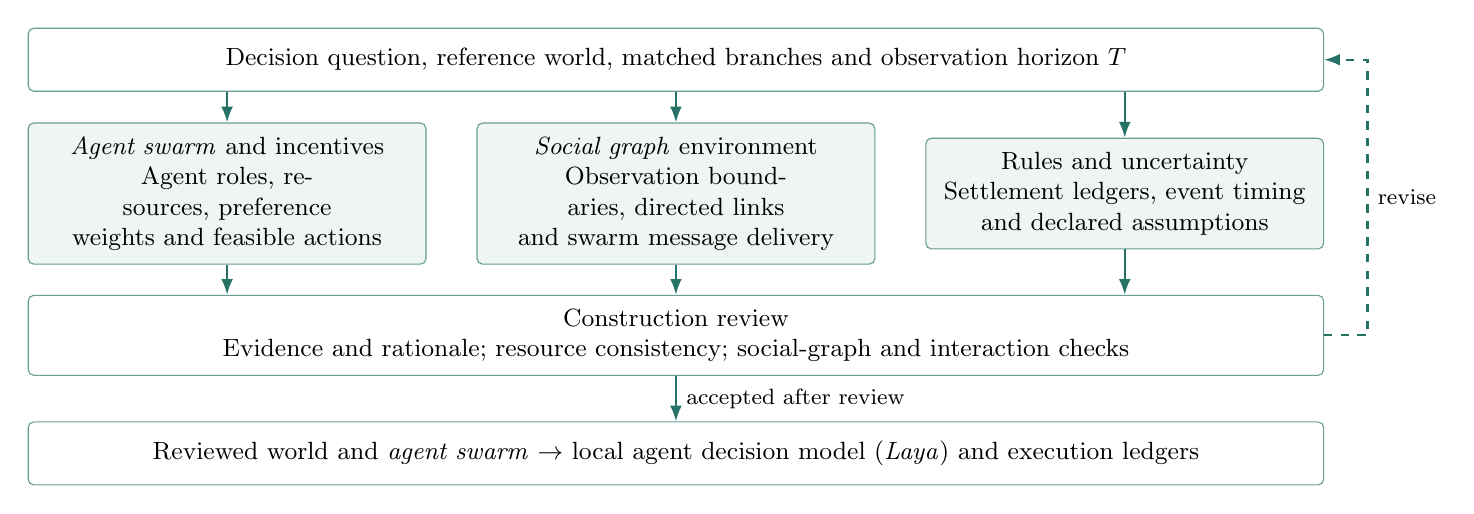
\begin{tikzpicture}[
 constructionbox/.style={draw=teal!70,fill=wash,rounded corners=2pt,align=center,text width=4.7cm,minimum height=1.15cm,inner sep=5pt,font=\small},
 wide/.style={draw=teal!70,fill=white,rounded corners=2pt,align=center,text width=16.1cm,minimum height=0.8cm,inner sep=5pt,font=\small},
 connection/.style={-{Latex[length=2mm]},thick,draw=teal}]
\node[wide] (question) at (5.7,0) {Decision question, reference world, matched branches and observation horizon $T$};
\node[constructionbox] (actors) at (0,-1.7) {\textit{Agent swarm} and incentives\\Agent roles, resources, preference\\weights and feasible actions};
\node[constructionbox] (information) at (5.7,-1.7) {\textit{Social graph} environment\\Observation boundaries, directed links\\and swarm message delivery};
\node[constructionbox] (rules) at (11.4,-1.7) {Rules and uncertainty\\Settlement ledgers, event timing\\and declared assumptions};
\draw[connection] (question.south -| actors.north)--(actors.north);
\draw[connection] (question.south)--(information.north);
\draw[connection] (question.south -| rules.north)--(rules.north);
\node[wide] (review) at (5.7,-3.5) {Construction review\\Evidence and rationale; resource consistency; social-graph and interaction checks};
\draw[connection] (actors.south)--(actors.south |- review.north);
\draw[connection] (information.south)--(review.north);
\draw[connection] (rules.south)--(rules.south |- review.north);
\node[wide] (output) at (5.7,-5) {Reviewed world and \textit{agent swarm} $\rightarrow$ local agent decision model (\textit{Laya}) and execution ledgers};
\draw[connection] (review.south)--node[right,font=\footnotesize]{accepted after review}(output.north);
\draw[connection,dashed] (review.east)--++(0.55,0)|-node[pos=0.25,right,font=\footnotesize]{revise}(question.east);
\end{tikzpicture}
\caption{\rev{World and \textit{agent swarm} construction in \textit{Boyun},
inspired by \textit{MiroFish}'s world-building workflow.} A decision question
determines three complementary specification tasks \rev{defining the swarm of
agents, their social graph, and the settlement rules}. Their outputs undergo
structural checks and human review, with author-directed revision where needed.
The process specifies \rev{agent preference weights, social-graph links, and
settlement rules before \textit{Laya} selects live agent actions locally.}}
\label{fig:construction}
\end{figure*}

\section{Problem Formulation and World Creation}\label{sec:world-creation}
The preceding section identified the conceptual foundations needed to study
strategic interactions. To turn those foundations into a reproducible
experiment, \rev{\textit{Boyun}---following \textit{MiroFish}'s world-first
workflow---}constructs a \textit{world}: an explicit specification of \rev{an
\textit{agent swarm} (modeled actors operating as autonomous agents)},
resources, \rev{a \textit{social graph} governing observations and communication},
actions, events, and settlement rules. Construction is performed by a user or a
separate authoring model, followed by structural checks and human review, and
finishes before the \rev{agent decision model} is ever called.
Figure~\ref{fig:construction} summarizes this preparation; the execution
procedure follows in Section~\ref{sec:method-system}.

\subsection{Core Terminology}
Before specifying a world, a reader must distinguish the static specification
from the record produced by executing it. Table~\ref{tab:definitions} defines
worlds and their execution, while actor and decision terms appear in the
subsections below. In particular, a world is a model of a decision setting,
whereas a run is one execution of that model; two runs of the same world can
differ whenever the selection rule uses sampling. For an everyday
analogy, a board game's rules and starting setup define the world, whereas one
played game is a run and its recorded move sequence is a trajectory.

\begin{table}[H]
\caption{Worlds and execution terminology.}
\label{tab:definitions}
\centering\small
\renewcommand{\arraystretch}{1.12}
\begin{tabularx}{\columnwidth}{@{}>{\raggedright\arraybackslash}p{0.25\columnwidth}Y@{}}
\toprule
Term & Definition \\
\midrule
\textit{World} & A specified decision setting: actors, resources, observations, actions, events, and settlement rules. \\
\textit{Scenario} & An alternative setting examined through a world or matched branch; its label does not establish a probability. \\
\textit{State} & Ledger-specific data at step $t$: balances and metrics, plus reserves, collateral, debt, or claims where modeled. \\
\textit{Run / trajectory} & A run executes one world. Its trajectory records observations, actions, and settled states. \\
\textit{Round / horizon} & Index $t$ orders rounds or decision points up to $T$; elapsed time is recorded separately. A cycle is not inherently an hour or day. \\
\textit{Outcome / metric} & An outcome is a simulated result. A metric $x_{k,t}$ describes shared state within bounds $[L_k,H_k]$; metric points are not money. \\
\bottomrule
\end{tabularx}
\end{table}

Once those terms are separated, the author can state what the simulation
is designed to compare. Consequently, world creation begins with the decision
question rather than with narrative persona writing.

\subsection{Decision Question, Alternatives, and Horizon}
Specifically, the author first defines the focal decision, the alternatives
under comparison, the observation horizon $T$, and the outcomes of interest.
For example, a protocol designer might compare early reserve disclosure against
delayed disclosure and track partner participation alongside retained cash.
That question dictates which actors and ledgers belong in the world; adding
unrelated detail does not strengthen the comparison.

From that focal question, the author defines a reference world and
isolates which inputs change in each matched branch. Comparing disclosure
policies, for instance, keeps initial balances and unrelated rules fixed
wherever possible; if several inputs change together, the resulting difference
reflects their joint intervention rather than a single cause. Likewise,
the horizon $T$ bounds only the observation window: reaching $T$ does not imply
that the modeled protocol or market has ended.

\subsection{\rev{Agent Swarm}, Preference Weights, and Strategic Dependence}
With the comparison fixed, \rev{agents enter the \textit{swarm} (the world's
cast)} only if they control relevant resources, hold distinct information, or
can alter an outcome that another \rev{agent} values. An \rev{\textit{actor} in
\textit{Boyun} is an autonomous modeled \textit{agent}}, while a
\textit{persona} describes its role and motivation. To make that persona
executable \rev{within the \textit{swarm of agents}}, the world assigns explicit
goals, initial balances, feasible actions, \rev{social-graph} observation
access, and numeric preference weights, giving the \rev{agent swarm} a
game-theoretic structure rather than a list of biographies
\cite{polak2,nash1950}. Table~\ref{tab:actor-definitions} separates these
elements.

\begin{table}[H]
\caption{\rev{Agent swarm, goals, and incentives.}}
\label{tab:actor-definitions}
\centering\small
\renewcommand{\arraystretch}{1.12}
\begin{tabularx}{\columnwidth}{@{}>{\raggedright\arraybackslash}p{0.25\columnwidth}Y@{}}
\toprule
Term & Definition \\
\midrule
\rev{\textit{Actor / agent}} & \rev{An autonomous modeled decision-maker indexed by $i$ (a player in game theory); the interacting collection of agents forms the \textit{agent swarm} (or \textit{cast}).} \\
\textit{Persona} & The \rev{agent's} descriptive role and motivation, paired with explicit preference weights and actions. \\
\textit{Goal} & The outcome the \rev{agent} seeks, distinct from the analyst's research question. \\
\textit{Incentive} & A cost, benefit, or conditional effect that makes an action more or less attractive under the \rev{agent's} preference weights. \\
\textit{Preference weights / utility} & In the strategic ledger, declared weights $w_{i,\mathrm{cash}},w_{i,k}$ map cash and metrics to utility $U_{i,t}$; utility need not equal profit. \\
\textit{Resource / constraint} & An available balance (such as cash $b_{i,t}$) and an enforced limit excluding unaffordable actions. \\
\bottomrule
\end{tabularx}
\end{table}

For instance, consider a partner deciding whether to fund a pilot. The
partner is an actor whose goal is preserving capital while gaining credible
participation; its preference weights quantify that trade-off, whereas action
costs and credibility gains create incentives. Funding and waiting are actions,
and selecting one from the actor's observation is a decision whose consequences
the ledger settles. This example illustrates how the terms connect rather than
claiming empirical partner behavior.

Moreover, within the same cast, actors can assign different preference
weights to retained cash, participation, credibility, or a declared risk
metric. The author must state what each metric represents and why its weight
reflects an assumed trade-off, because calling a persona ``cautious'' in prose
does not enforce caution in settlement. In everyday terms, \textit{utility}
resembles commuters ranking routes: one commuter weights a lower fare more
heavily, whereas another weights a shorter trip, so different choices emerge
without assuming everyone minimizes fare.

Beyond individual preference weights, strategic dependence requires rules
that couple actors' choices. Supporting a launch may pay off only if an
independent reviewer verifies it, or two simultaneous actions may shift a
shared metric more than the sum of their individual effects. However, a
promise or threat in persona text has no binding force unless an executable
rule enforces it. Similarly, splitting one actor cohort into multiple accounts
requires partitioning its balances and per-action effects rather than copying
its full market power into each new account.

\subsection{\rev{Social Graph}, Information, Rules, and Event Timing}
Alongside incentives, each \rev{agent in the swarm} operates behind an explicit
observation boundary \rev{defined by a \textit{social graph}}. Directed edges in
the \rev{\textit{social graph} (implemented as an \textit{information graph})
determine how agents in the swarm communicate and whose messages an agent
receives}, while the engine withholds other \rev{agents'} private preference
weights and unannounced future events. In the strategic ledger, messages
attached to round-$t$ actions arrive in round $t+1$, ensuring that query order
within a round never grants an unintended information advantage. By analogy, an
\textit{observation} is a card player's view of their own hand and public table
cards, whereas \rev{the swarm's \textit{social graph}} works like mailing-list
subscriptions, which need neither be mutual nor imply trust.
Table~\ref{tab:decision-definitions} summarizes these terms.

\begin{table}[H]
\caption{\rev{Decisions, social-graph observations, and rules.}}
\label{tab:decision-definitions}
\centering\small
\renewcommand{\arraystretch}{1.12}
\begin{tabularx}{\columnwidth}{@{}>{\raggedright\arraybackslash}p{0.25\columnwidth}Y@{}}
\toprule
Term & Definition \\
\midrule
\textit{Action} & A permitted option $a \in \operatorname{Menu}_i$ with declared cost $c_i(a)$, effects, and optional preset message; \texttt{wait} is an action. \\
\textit{Decision} & Selection of an affordable action $a_{i,t} \in A_{i,t}$ from \rev{agent} $i$'s observation; the ledger settles consequences separately. \\
\textit{Observation} & Information visible to one \rev{agent} at $t$: its own profile and balances, public state, visible events, and delivered \rev{social-graph} messages. \\
\rev{\textit{Social / information graph}} & \rev{Directed communication network through which the \textit{swarm of agents} exchanges messages, specifying permitted delivery rather than measuring social influence.} \\
\textit{Event} & An exogenous change with declared timing, audience visibility, and state effects. \\
\textit{Rule / interaction} & A settlement law; in the strategic ledger, a joint-action rule $r$ adds effect $g_{k,r}$ when a specified action combination occurs. \\
\bottomrule
\end{tabularx}
\end{table}

To settle choices consistently, the world also declares action costs,
metric bounds $[L_k,H_k]$, ledger parameters, and exogenous event schedules.
Default strategic worlds apply deterministic event schedules, whereas
probabilistic event trees belong to a separate event-chain module. Keeping
exogenous events distinct from endogenous actor actions lets later analysis
trace whether a trajectory shift came from an external shock or from cast
reactions.

\subsection{Evidence, Assumptions, and Uncertainty}
Because settlement rules fix the meaning of every simulated number, each
material parameter must trace back to cited evidence or a labeled assumption.
An \textit{assumption} is an unverified modeling input, whereas
\textit{evidence} is a dated external record motivating part of the world. For
example, a parliamentary agenda may establish the date of a debate without
establishing how traders will react; world construction therefore records the
dated source and the assumed behavioral response separately, following
established model-documentation practice \cite{grimm2020}.

On the other hand, whenever a scenario introduces numerical probabilities,
the author must distinguish a user-chosen scenario branch, a model-returned
option score $q_{i,t}(a)$, a seeded sampling draw, and an empirical frequency.
In particular, \textit{Bayesian} updating requires declared hypotheses, priors,
and likelihoods \cite{pishronik2014} rather than inferring odds from narrative
text; uncalibrated scenario weights are therefore reported strictly as
assumptions.

\subsection{Construction Review and Output}
Before any run starts, automated checks and human review audit the assembled
world. Specifically, construction checks verify balance conservation, metric
units, affordable action menus, isolated unilateral deltas, information links,
and joint-action couplings, flagging degenerate setups such as actors with only
one affordable option or goals unaffected by any permitted action.

Consequently, passing construction review guarantees an explicit,
executable specification rather than an empirically calibrated population;
human judgment remains responsible for checking whether preference weights match
intended roles and whether cited sources justify the parameters. With that
specification frozen, Section~\ref{sec:method-system} details how
\textit{Boyun} executes rounds and decision points locally.

\begin{figure*}[!t]
\centering
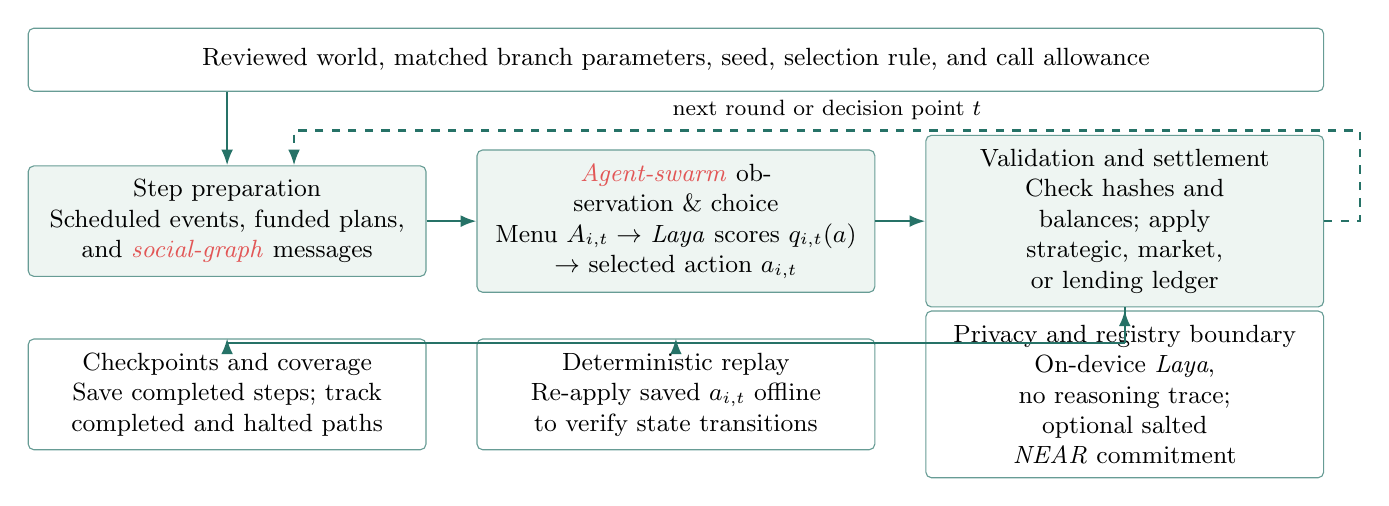
\begin{tikzpicture}[
 stagebox/.style={draw=teal!70,fill=wash,rounded corners=2pt,align=center,text width=4.7cm,minimum height=1.3cm,inner sep=5pt,font=\small},
 boundarybox/.style={draw=teal!70,fill=white,rounded corners=2pt,align=center,text width=4.7cm,minimum height=1.25cm,inner sep=5pt,font=\small},
 wide/.style={draw=teal!70,fill=white,rounded corners=2pt,align=center,text width=16.1cm,minimum height=0.8cm,inner sep=5pt,font=\small},
 connection/.style={-{Latex[length=2mm]},thick,draw=teal}]
\node[wide] (input) at (5.7,0) {Reviewed world, matched branch parameters, seed, selection rule, and call allowance};
\node[stagebox] (prep) at (0,-2.05) {Step preparation\\Scheduled events, funded plans,\\and \rev{\textit{social-graph}} messages};
\node[stagebox] (choice) at (5.7,-2.05) {\rev{\textit{Agent-swarm}} observation \& choice\\Menu $A_{i,t} \rightarrow$ \textit{Laya} scores $q_{i,t}(a)$\\$\rightarrow$ selected action $a_{i,t}$};
\node[stagebox] (settle) at (11.4,-2.05) {Validation and settlement\\Check hashes and balances; apply\\strategic, market, or lending ledger};
\draw[connection] (input.south -| prep.north)--(prep.north);
\draw[connection] (prep.east)--(choice.west);
\draw[connection] (choice.east)--(settle.west);
\draw[connection,dashed] (settle.east)--++(0.45,0)--++(0,1.15)-|node[pos=0.25,above,font=\footnotesize]{next round or decision point $t$}([xshift=0.85cm]prep.north);
\node[boundarybox] (ckpt) at (0,-4.25) {Checkpoints and coverage\\Save completed steps; track\\completed and halted paths};
\node[boundarybox] (replay) at (5.7,-4.25) {Deterministic replay\\Re-apply saved $a_{i,t}$ offline\\to verify state transitions};
\node[boundarybox] (boundary) at (11.4,-4.25) {Privacy and registry boundary\\On-device \textit{Laya}, no reasoning trace;\\optional salted \textit{NEAR} commitment};
\coordinate (split) at ([yshift=-0.45cm]settle.south);
\draw[thick,draw=teal] (settle.south)--(split);
\draw[connection] (split)-|(ckpt.north);
\draw[connection] (split)-|(replay.north);
\draw[connection,dashed] (split)--(boundary.north);
\end{tikzpicture}
\caption{Simulation pipeline and evidence boundaries in \textit{Boyun}.
At each round or decision point $t$, the engine prepares exogenous updates \rev{and \textit{social-graph} deliveries},
builds per-agent observations \rev{across the \textit{swarm of agents}}, obtains option scores $q_{i,t}(a)$ locally from
\textit{Laya} (or an explicit offline baseline), and settles transitions on the
active ledger. Option scores $q_{i,t}(a)$, selected actions $a_{i,t}$, and
settled states remain distinct in the saved record; dashed arrows denote
continuation up to horizon $T$ and optional on-chain commitment.}
\label{fig:execution-pipeline}
\end{figure*}

\section{Simulation Method and System Design}\label{sec:method-system}
Section~\ref{sec:world-creation} ended with a reviewed world specification;
this section explains how \textit{Boyun} executes it \rev{across a \textit{swarm of agents}}. Returning to the
board-game analogy, world creation fixes the rules and opening balances, while
execution plays the game one step at a time. At each step $t$, the engine
shows every \rev{agent} $i$ \rev{in the \textit{agent swarm}} only its permitted observation \rev{along the \textit{social graph}}, queries the local
actor decision model (\textit{Laya}) over the actions that \rev{agent} $i$
can afford, and settles all selected actions on a deterministic ledger.
Consequently, the model selects moves \rev{for each agent in the swarm} but can never alter permissions or
accounting. Figure~\ref{fig:execution-pipeline} summarizes this pipeline. After
fixing the execution terms (Section~\ref{sec:exec-terms}), we trace \rev{\textit{agent-swarm}} observation
construction, action selection, \rev{\textit{social-graph}} message and event timing, and settlement across
the strategic, market, and lending ledgers, followed by analytical
modules, replay, and self-hosted privacy boundaries.

\subsection{Execution Terminology}\label{sec:exec-terms}
To keep terminology consistent across all three ledgers,
Table~\ref{tab:execution-terms} defines the runtime concepts that complement
Tables~\ref{tab:definitions}--\ref{tab:decision-definitions}. Discrete
strategic worlds advance by \textit{rounds}, whereas timestamped market and
lending worlds advance by scheduled \textit{decision points}; both use an ordered index $t \in \{1,\dots,T\}$. The associated timestamp
$\tau_t$ records elapsed physical time. Hours and days in the case results
refer to $\tau_t$, not to the decision index; finer launch steps therefore do
not count as additional elapsed hours.

\begin{table}[H]
\caption{Execution terminology and notation.}
\label{tab:execution-terms}
\centering\small
\renewcommand{\arraystretch}{1.12}
\begin{tabularx}{\columnwidth}{@{}>{\raggedright\arraybackslash}p{0.27\columnwidth}Y@{}}
\toprule
Term & Definition \\
\midrule
\textit{Affordable action menu} $A_{i,t}$ & Feasible options for actor $i$ at step $t$. In the strategic ledger this filters the reviewed menu by cash $b_{i,t}$; market and lending menus use their own ledger constraints. \\
\textit{Option scores} $q_{i,t}(a)$ & Normalized weights in $[0,1]$ summing to 1 returned by the actor decision model over $A_{i,t}$; not empirical odds. \\
\textit{Selection rule} & Pre-declared rule (\textit{argmax} or \textit{sampling}) mapping $q_{i,t}(a)$ to one action $a_{i,t}$. \\
\textit{Settlement} & Atomic state transition applying chosen actions on the strategic, market, or lending ledger. \\
\textit{Matched branch} & Counterfactual run sharing initial state, seed, and schedule up to an intervention while varying one policy. \\
\textit{Checkpoint / replay} & Saved step state and offline re-execution of saved $a_{i,t}$ without calling the model to verify exact state agreement. \\
\bottomrule
\end{tabularx}
\end{table}

Among these concepts, deterministic replay is central to verification:
much like replaying a recorded chess game from algebraic notation, replay
re-applies saved moves without re-querying the player, so any mismatch isolates
a rule or accounting defect.

\subsection{\rev{Agent-Swarm} Observations and Affordable Actions}
Executing step $t$ begins by restricting what each \rev{agent} $i$ \rev{in the \textit{swarm of agents}} can see. If
every \rev{agent} observed rivals' private preference weights and future
events, choices would reflect the world author's omniscience rather than local
incentives \rev{across the \textit{social graph}}. For each \rev{agent} $i$, the engine constructs a canonical JSON
\textit{observation} containing its persona, goal, preference weights, and
pre-decision cash $b_{i,t}$; visible public state (such as shared metrics
$x_{k,t}$ indexed by $k$, pool reserves, or oracle prices); delivered
\rev{\textit{social-graph}} messages and visible events; and receipts from \rev{agent} $i$'s own
earlier actions, together with a SHA-256 observation hash. At the same
time, withholding private fields enforces an information boundary inside the
\rev{\textit{agent swarm}} rather than encrypting memory on the host machine.

Restricting information, however, does not by itself prevent overspending.
In the strategic ledger, before querying \textit{Laya}, code filters actor $i$'s reviewed menu
$\operatorname{Menu}_i$ against current cash $b_{i,t}$ to form the
\textit{affordable action menu}:
\begin{equation}
A_{i,t}=\{a\in\operatorname{Menu}_i : c_i(a)\leq b_{i,t}\},
\label{eq:affordable}
\end{equation}
where $c_i(a)$ is the integer cash cost of action $a$. Enforcing
Eq.~\eqref{eq:affordable} in code guarantees that affordability depends on
ledger balances rather than on how the model reads narrative text.

\subsection{Action Selection}\label{sec:action-selection}
Once $A_{i,t}$ is fixed, the engine selects exactly one action $a_{i,t}$.
In the strategic ledger, whenever only \texttt{wait} is affordable ($|A_{i,t}|=1$), no choice exists, so
the engine records \texttt{wait} without a model query. Otherwise, it passes
the hashed observation and a typed \texttt{Choice} prompt to \textit{Laya} on
the local CPU \cite{layamodel}. Other open-weight backends are a future
evaluation direction, not an inference result established here. In strategic worlds, each option is paired
with a code-computed unilateral projection of immediate post-action cash,
clamped metrics, and utility delta holding peer actions fixed, so arithmetic is
supplied by code rather than delegated to the model.

Because \textit{Laya} outputs option scores rather than state mutations,
the adapter validates every response before selection. Specifically, the
response must assign a finite score $q_{i,t}(a)\in[0,1]$ to each $a\in A_{i,t}$
with $\sum_{a\in A_{i,t}} q_{i,t}(a)=1$, identify a top-scoring action, and
include the model's confidence field; malformed responses halt the step without
partial settlement (allowing only a $\le 0.001$ rescaling tolerance for
\textit{Laya}'s four-decimal rounding).

Given a validated distribution, the pre-declared \textit{selection rule}
maps $q_{i,t}(a)$ to $a_{i,t}$ via either \textit{argmax} or seeded
\textit{sampling}:
\begin{align}
\text{argmax:}\quad & a_{i,t}=\arg\max_{a\in A_{i,t}} q_{i,t}(a),\label{eq:selection}\\
\text{sampling:}\quad & a_{i,t}=a_{(m^\ast)},\ \text{where}\notag\\
& m^\ast=\min\Big\{m:\textstyle\sum_{\nu=1}^{m} q_{i,t}\big(a_{(\nu)}\big)>\xi_{i,t}\Big\}.\label{eq:sampling}
\end{align}
Here $a_{(1)},a_{(2)},\dots$ order $A_{i,t}$ canonically, $\nu$ indexes the
cumulative sum, and $\xi_{i,t}\in[0,1)$ is a deterministic pseudorandom draw
keyed to the run seed and decision identity. Under Eq.~\eqref{eq:sampling}, an
action with score $0.30$ is drawn for $30\%$ of $\xi_{i,t}$ values while
remaining exactly reproducible across replays. Nevertheless, neither
selection rule turns $q_{i,t}(a)$ into an empirically calibrated probability or
a solved mixed-strategy Nash equilibrium \cite{nash1950,polak15}.

\subsection{\rev{Social-Graph} Messages, \rev{Swarm} Memory, and Event Timing}\label{sec:messages}
Beyond changing balances, $a_{i,t}$ can transmit information \rev{through the \textit{social graph} to other agents in the \textit{swarm of agents} at} later
steps. In the strategic ledger, a preset message attached to $a_{i,t}$ follows
the \rev{\textit{social graph} (\textit{directed information graph})} and arrives at subscribed \rev{agents} at the
start of round $t+1$; in timestamped ledgers, messages obey declared delivery
delays and recipient lists \rev{across the swarm}. Delaying delivery ensures that within-step
evaluation order never creates an artificial first-mover leak. Observations
also retain bounded memory of \rev{agent} $i$'s own prior actions and public state
history without exposing peers' private balances, while delivered \rev{\textit{social-graph}} messages
remain unverified claims unless backed by executable rules
\cite{polak15,polak18}.

On the other side, exogenous events and pre-committed plans enter on
explicit schedules separate from actor reactions. Strategic rounds apply
scheduled events before building round-$t$ observations, whereas timestamped
ledgers record both occurrence time and availability time to represent
reporting lag. Furthermore, when a scenario tests a funded launch or marketing
plan, committed actions execute and deduct payer cash at their scheduled
decision point before outside actors observe the result and choose $a_{i,t}$.

\subsection{Strategic Ledger Settlement and Accounting}\label{sec:settlement}
After all actors choose $a_{i,t}$ from the same frozen state, the
strategic ledger applies \textit{synchronous settlement} so actor ordering
cannot distort bounded metrics. First, the engine re-verifies every observation
hash and Eq.~\eqref{eq:affordable}; if any check fails, the round aborts
without mutating state. Otherwise, cash balances and shared metrics update
atomically:
\begin{align}
b^{+}_{i,t}&=b_{i,t}-c_i(a_{i,t}),\label{eq:cash-update}\\
x^{+}_{k,t}&=\operatorname{clip}_{[L_k,\,H_k]}\Big(x_{k,t}+\sum_{i}e_{k}(a_{i,t})+\sum_{r\in R_t}g_{k,r}\Big),\label{eq:settlement}
\end{align}
where $e_k(a)$ is action $a$'s effect on metric $k$, $R_t$ is the set of
joint-action rules triggered at round $t$, $g_{k,r}$ is rule $r$'s effect on
metric $k$, and $\operatorname{clip}_{[L,H]}(z)=\min(H,\max(L,z))$ enforces
bounds once after summing all effects. The superscript $+$ denotes the
post-settlement state of this round; scheduled events for the next round are
applied afterward to construct its observation state. Algorithm~\ref{alg:round} summarizes the
strategic-round loop and offline replay. Timestamped ledgers have their own
execution procedures; this algorithm is not a shared implementation for all
three ledgers.

\begin{algorithm}[t]
\caption{Strategic-round execution, synchronous settlement, and replay}
\label{alg:round}
\footnotesize
\begin{algorithmic}[1]
\Require Reviewed strategic world, selection rule, seed, call allowance
\State Validate cast, balances, bounds, events, and information graph
\For{each strategic round $t=1,\dots,T$}
  \State Apply scheduled events and funded commitments; deliver prior messages
  \State Freeze pre-decision state and build hashed observations
  \For{each actor $i$}
    \State Form $A_{i,t}$ by Eq.~\eqref{eq:affordable}
    \If{$|A_{i,t}|=1$}
      \State Set $a_{i,t}\gets\texttt{wait}$ without querying \textit{Laya}
    \Else
      \State Query local \textit{Laya} (or offline baseline) within call allowance
      \State Validate $q_{i,t}(a)$; select $a_{i,t}$ via Eq.~\eqref{eq:selection} or~\eqref{eq:sampling}
    \EndIf
  \EndFor
  \If{any observation hash or action $a_{i,t}$ is invalid}
    \State Reject step $t$ without mutating state; \textbf{stop}
  \EndIf
  \State Settle the strategic state; save receipts and checkpoint
\EndFor
\State Re-apply saved $a_{i,t}$ offline without \textit{Laya}; verify identical states
\end{algorithmic}
\end{algorithm}

To evaluate settled strategic states across heterogeneous roles, actor
$i$'s utility combines retained cash and metrics via its declared preference
weights:
\begin{equation}
U_{i,t} = w_{i,\mathrm{cash}}\, b_{i,t} + \sum_k w_{i,k}\, x_{k,t}.
\label{eq:utility}
\end{equation}
Here $U_{i,t}$ is the strategic ledger's preference measure, not dollar profit.
Weights carry the units needed to convert cash and metric units into the
chosen utility scale. This linear formula is not an estimated investor utility
function and does not define a common utility calculation for the market and
lending ledgers.
In addition, because Eq.~\eqref{eq:affordable} bounds $c_i(a_{i,t})\le
b_{i,t}$ and Eq.~\eqref{eq:cash-update} adds each integer deduction to
cumulative cast spending $S_t^{+}$ through settlement of round $t$, every
settled round satisfies exact cash conservation:
\begin{equation}
b^{+}_{i,t}\geq 0 \quad\text{and}\quad \sum_i b^{+}_{i,t}+S_t^{+}=\sum_i b_{i,0}.
\label{eq:conservation}
\end{equation}

\subsection{Market Ledger}\label{sec:market}
Whereas the strategic ledger treats cumulative spending $S_t^{+}$ as effort leaving the cast,
market scenarios require counterparty fills, reserves, and prices. The market
ledger tracks integer cash and tokens and settles swaps using a simplified
constant-product automated market maker (AMM) \cite{angeris2021,xu2023amm}.
A swap's output depends on reserves, the configured fee, and integer rounding;
pre-migration phases use specified virtual reserves \cite{pumpdocs}.
Orders outside slippage or inventory limits are rejected atomically with a
recorded reason. This execution model is a stated approximation, not a complete
implementation of a live venue. Reports distinguish realized cash from the
quoted value of unsold inventory.

\subsection{Lending Ledger}\label{sec:lending}
Complementing spot trading, protocol credit decisions require tracking
deposits, collateralized debt, and liquidations on a separate \textit{lending
ledger}. \textit{Suppliers} deposit stablecoins into a pool with idle cash
$C_t$ and lent principal $P_t$, holding claims $c_s$ (withdrawals exceeding
$C_t$ wait in a first-in, first-out queue ahead of new loans), while
\textit{borrowers} pledge volatile collateral against loans indexed by $\ell$.
With pool \textit{utilization} $u_t=P_t/(C_t+P_t)$, the annual borrow rate
follows the standard kinked rate model \cite{gudgeon2020}:
\begin{equation}
r(u_t)=\begin{cases}
r_0+(r^\ast-r_0)\,u_t/u^\ast, & u_t\le u^\ast,\\
r^\ast+(r_1-r^\ast)\,(u_t-u^\ast)/(1-u^\ast), & u_t>u^\ast,
\end{cases}
\label{eq:rate}
\end{equation}
where $r_0$ is the base rate, $u^\ast$ is the kink utilization, $r^\ast$ is
the rate at $u^\ast$, and $r_1$ is the full-utilization rate. Over $\Delta t$
seconds ($Y$ seconds per 365-day year), loan $\ell$ incurs simple interest
$I_\ell=P_\ell\,r(u_t)\,\Delta t/Y$, accruing to the protocol (share $\varphi$)
and each supplier $s$:
\begin{equation}
\Delta I^{\mathrm{prot}}_\ell=\big\lfloor \varphi\, I_\ell\big\rfloor_{\epsilon},\qquad
\Delta I^{s}_\ell=\Big\lfloor (1-\varphi)\, I_\ell\,\frac{c_s}{\sum_{s'}c_{s'}}\Big\rfloor_{\epsilon},
\label{eq:accrual}
\end{equation}
rounded down to $\epsilon=10^{-12}$ stablecoin units. Specifically, this
fixed grid bounds arithmetic precision over repeated hourly accruals while
keeping interest allocation within the declared rounding rules.

Meanwhile, solvency is governed by each loan $\ell$'s \textit{health
factor} \cite{aaveliquidations}:
\begin{equation}
h_\ell=\frac{Q_\ell\,p_t\,\theta}{D_\ell\,p^{\mathrm{usd}}_t},
\label{eq:health}
\end{equation}
where $Q_\ell$ is pledged collateral at oracle price $p_t$, $\theta$ is the
liquidation threshold, and $D_\ell$ is principal plus accrued interest at
stablecoin price $p_t^{\mathrm{usd}}$. When $h_\ell<1$, a liquidator repays
debt (partially, or fully once $h_\ell\le 0.95$) for collateral worth $1+\beta$
times repayment, executed only if net market proceeds cover repayment and costs;
residual underwater debt writes off against a capped loss reserve, and stale
oracle timestamps halt borrowing and liquidations.

\subsection{Analytical Modules}\label{sec:analysis}
Apart from time-stepped ledgers, \textit{Boyun} provides three standalone
analytical modules that operate strictly on user-supplied inputs. First, for
small normal-form games ($\le 4$ actors and $\le 256$ profiles) with exact
payoffs $U_i(a_i,a_{-i})$ and supplied opponent beliefs $\pi_i(a_{-i})$,
code computes expected utility, regret, and pure-strategy Nash equilibria
\cite{nash1950}:
\begin{align}
\mathrm{EU}_i(a_i)&=\textstyle\sum_{a_{-i}}\pi_i(a_{-i})\,U_i(a_i,a_{-i}),\label{eq:eu}\\
\mathrm{Reg}_i(a_i)&=\textstyle\max_{a'}\mathrm{EU}_i(a')-\mathrm{EU}_i(a_i).\label{eq:regret}
\end{align}
Second, for finite hypothesis sets $H$ with supplied priors $P(h)$ and signal
likelihoods $P(E\mid h)$, \textit{Bayesian updating} computes
\cite{pishronik2014}
\begin{equation}
P(h\mid E)=\frac{P(E\mid h)\,P(h)}{\sum_{h'\in H}P(E\mid h')\,P(h')}.
\label{eq:bayes}
\end{equation}
Third, seeded \textit{Monte Carlo} batches summarize declared branch outcomes
via nearest-rank quantiles (5th, 50th, and 95th percentiles), describing batch
dispersion rather than empirical market confidence intervals.

\subsection{Matched Branches, Checkpoints, Replay, and Privacy}\label{sec:boundaries}
To isolate policy effects across any ledger, \textit{matched branches}
hold opening balances, seeds, and exogenous schedules identical while changing
one policy rule. Checksummed \textit{checkpoints} persist every settled step
(and, in the lending runner, an append-only request-keyed decision cache) so
interrupted local runs resume without repeating completed work. Afterward,
\textit{replay} re-runs the saved actions $a_{i,t}$ through the hash-pinned
engine without calling \textit{Laya} to verify bit-identical state trajectories.

Finally, self-hosted execution defines \textit{Boyun}'s cost, privacy, and
auditability profile. Running \textit{Laya} locally incurs zero API fees and
avoids sending actor observations to a hosted inference endpoint. This claim
remains scoped to the local inference path: external data requests, artifact
sharing, optional on-chain commitments, and host access are separate privacy
boundaries. In exchange, \textit{Laya} enforces a 1024-token context ceiling
(truncating inputs are rejected) and exposes no internal chain of thought
\cite{layamodel}. For no-API baselines and external agent workflows, a
deterministic immediate-utility rule and a local stdio \textit{Model Context
Protocol} (MCP) server \cite{mcp2025} run completely offline. When tamper
evidence is needed prior to disclosure, an optional \textit{cryptographic
commitment} hashes the artifact with a fresh 32-byte salt via SHA-256 and
records the digest on \textit{NEAR} testnet \cite{nearprotocol,nightshade2024},
binding timestamped integrity without certifying behavioral realism.
Section~\ref{sec:evaluation} designs the experiments that test these
capabilities and boundaries.

\section{Evaluation Design}\label{sec:evaluation}
Section~\ref{sec:method-system} specified how \textit{Boyun} executes a world;
this section specifies how we test whether that execution does what it claims
and what it adds in practice. Two kinds of test are needed, and they answer
different questions. \textit{Verification} asks whether the program carries
out the stated rules correctly. \textit{Validation} asks whether those rules
and the model's choices resemble real actors and markets. The tests
below are mainly verification and capability tests; none of them validates
\textit{Boyun} as a forecaster, and the results in Section~\ref{sec:results}
are interpreted accordingly.

\subsection{Research Questions}
Given that boundary, the evaluation addresses six research questions (RQs),
ordered from the most controlled test to the most open comparison:
\begin{enumerate}\setlength{\itemsep}{1pt}
\item[\textit{RQ1}] Do the implemented calculations, timing, accounting, and
replay match their specifications in Section~\ref{sec:method-system}?
\item[\textit{RQ2}] Do information delivery, joint rules, and numeric
preferences have separate and inspectable effects on choices and outcomes?
\item[\textit{RQ3}] Can a fourteen-day financial case with sixteen actors run
with settled trades, recorded rejections, matched policy branches, replay,
and a bounded budget, and what does it record?
\item[\textit{RQ4}] Given the same brief, what does \textit{Boyun} record that
the original \textit{MiroFish} does not, and what does \textit{MiroFish}
provide that \textit{Boyun} lacks?
\item[\textit{RQ5}] What do the local model's score distributions and
regime responses reveal about the limits of its simulated behavior?
\item[\textit{RQ6}] In a ninety-day lending launch, which observations follow
from explicit rules and which depend on unvalidated actor choices?
\end{enumerate}

\subsection{Synthetic Mechanism Experiments}\label{sec:eval-synthetic}
The first two questions require tests whose correct answers are known in
advance. Six small synthetic experiments provide them
(Table~\ref{tab:experiments}). Each uses invented inputs, and wherever an
action is needed it uses a fixed policy rather than a model, so any
discrepancy must come from the engine. No model is called and network access
is disabled while they run. Experiments~1, 2, and~4 test the analytical tools
and scoring formulas against hand calculations; Experiment~3 tests timing,
accounting, and replay; Experiments~5 and~6 address RQ2 by switching single
mechanisms on and off. These experiments are complemented by the engine's
automated test suite.

\begin{table}[H]
\caption{Synthetic mechanism experiments.}
\label{tab:experiments}
\centering\small
\renewcommand{\arraystretch}{1.12}
\begin{tabularx}{\columnwidth}{@{}>{\raggedright\arraybackslash}p{0.07\columnwidth}>{\raggedright\arraybackslash}p{0.27\columnwidth}Y@{}}
\toprule
Exp. & Mechanism & Known answer checked \\
\midrule
1 & Game analysis & Expected utility, regret, and pure Nash profiles, Eqs.~\eqref{eq:eu}--\eqref{eq:regret} \\
2 & Bayesian updating & Two sequential posteriors, Eq.~\eqref{eq:bayes} \\
3 & Timing and accounting & Event order, clipping, conservation, replay, Eqs.~\eqref{eq:cash-update}--\eqref{eq:conservation} \\
4 & Forecast scoring & Brier and log scores against a baseline, Eqs.~\eqref{eq:brier}--\eqref{eq:logloss} \\
5 & Communication ablation & Delivery and a joint rule switched on and off \\
6 & Preferences vs.\ prose & Changing a weight versus changing persona text \\
\bottomrule
\end{tabularx}
\end{table}

\subsection{MACRON Case Study}\label{sec:eval-macron}
Synthetic checks cannot show whether the engine copes with a realistic case,
so RQ3 uses \textit{MACRON}, a prospective fourteen-day launch of a
hypothetical political memecoin on a \textit{Solana} launch venue, beginning
2 November 2026. A founder with \$50{,}000 of capital, of which \$10{,}000 is a
protected reserve, launches the token on a bonding curve that later migrates
to a pool (Section~\ref{sec:market}). Sixteen actors take part: the founder, a
market maker, four retail traders with different strategies, a large buyer, an
attention trader, four promoters, a meme curator, an organic supporter, a
campaign operator, and a foundation. Each receives its own state, the public
market history, and only the private instructions it is permitted to see.
Real dated events, such as scheduled parliamentary sessions, enter as
exogenous events, without assuming their outcomes.

The case compares founder plans in a full factorial design. The founder's
initial position is \$5{,}000, \$10{,}000, or \$15{,}000; upfront marketing and
operating costs are \$5{,}000 or \$10{,}000; the market regime is
\textit{BULL} or \textit{BEAR}; and the response to an exit alert is either
\textit{pause-and-observe}, which stops discretionary spending and keeps the
tokens, or \textit{staged exit}, which sells in tranches. The regimes are
hypotheses about risk appetite, not observed market states. The resulting
$3\times2\times2\times2=24$ paths run hourly for up to 336 hours, with finer
steps around the launch. Each path uses one seed, so the design compares plans
under common conditions rather than sampling a population of outcomes. \begin{revised}
All 24 paths use local \textit{Laya} inference from hour 0 to hour 336.
No hosted-model decisions or mixed-model continuations enter these case results.
The packages, seeds, response policies, and evidence registers are fixed before
execution. Offline reference paths remain engineering checks rather than
substitutes for these model-driven paths.
\end{revised}

\subsection{Comparison with \textit{MiroFish}}\label{sec:eval-mirofish}
Because \textit{Boyun} was inspired by \textit{MiroFish}, RQ4 compares the two
on the same case. The original \textit{MiroFish} (source revision
\texttt{7657031}) \cite{mirofish} received the same frozen \textit{MACRON}
brief and event calendar, generated its sixteen personas with its own native
prompts, and ran its social simulation on the \textit{OASIS} platform
\cite{yang2025} for 336 hourly rounds in each regime, followed by its own
report generation. It used \textit{Gemini} 3.5 Flash-Lite on free quotas.
Interruptions caused by quota limits required restoring the saved actor
memories and databases; the original random state could not be recovered and
was reseeded, so the run is a declared recovery-adapted version rather than
an uninterrupted stock run.

The comparison is therefore matched in its inputs but not in everything else.
The two systems use different actor models, budgets, and actor activation
rules, and they are designed to produce different kinds of output, social
posts in one case and settled trades in the other. We therefore compare what
each system records and reports, rather than ranking them on a single score,
and we make no claim that either forecasts the real launch.

\subsection{Local Actor Behavior}\label{sec:eval-laya}
\begin{revised}
Beyond completion, RQ5 examines how local actor scores translate into
observed behavior. We report score concentration, filled and rejected trades,
and differences between the declared \textit{BULL} and \textit{BEAR} regimes.
The lifecycle engine samples actions from the saved score distributions;
therefore a weak preference between options can produce substantial turnover.
These are descriptive diagnostics of this model and selection rule, not a
calibration study or a measure of real investor behavior.
\end{revised}

\subsection{NEAR Lending Case Study}\label{sec:eval-lending}
Apart from token trading, RQ6 changes the financial mechanism to collateralized
lending, retaining local \textit{Laya} inference. Its case
is a prospective launch of a lending market on \textit{NEAR} that accepts
native NEAR as collateral and lends Circle's native USDC, evaluated over its
first 90 days. The world was built with the user through 41 recorded answers.
Because no partner terms had been negotiated, the user chose to assume that
\$1{,}000{,}000 of USDC from friendly partners is already deposited at
opening. The team holds \$100{,}000, of which \$10{,}000 is a capped loss
reserve, and suppliers earn points only on USDC that is actually borrowed.
Twenty decision-makers take part: the team, four friendly partners, two large
independent suppliers and two supplier groups, four borrowers and one
borrower group, an actor who both supplies and borrows to earn points,
two liquidators, and three distribution partners. Their balances are
synthetic, sized against the user's premises and a dated snapshot of
\textit{RHEA}, the main existing NEAR lending venue, which paid 9.88\% a year to
native-USDC suppliers and charged borrowers 15.29\% \cite{rhealending}. Every
actor sees these rates as a fixed outside option.

Within that cast, the rules of Section~\ref{sec:lending} apply with a 50\%
maximum loan-to-value, liquidation at 65\%, a 5\% liquidation bonus, a
\$500{,}000 aggregate borrowing cap, and, in the baseline, a \$50{,}000 cap per
borrower. Outsiders can act only after a channel they follow delivers a
campaign item; paid partners may accept, delay, or decline, and cash is spent
only on delivery, so no conversion rate is assumed. The ledger settles hourly,
and actors who are aware of the launch decide daily and whenever a trigger
fires, such as a NEAR price move of 8\% within 24 hours. Prices are real
hourly closes from Binance \cite{binanceklines}, rescaled so that each window
opens at the snapshot price: a choppy window beginning 12 August 2025, which
contains the market-wide fall of 10 October 2025, and a bear window beginning
9 November 2025.

\begin{revised}
These inputs define four local \textit{Laya} worlds
(Table~\ref{tab:lending-design}). Codes identify the price path (C for choppy,
B for bear), per-borrower cap in thousands of dollars, rate curve, and local
model. Each world has one seed and there is no no-launch arm; real-world odds
are unknown. Raising the cap also splits a borrower cohort, so that comparison
changes two design factors and does not isolate the cap alone.
\end{revised}

\begin{table}[t]
\caption{\rev{Local \textit{Laya} lending worlds.} R2: 2\% base rate, 10\% at 80\% utilization,
50\% at full use. R8: 8\% base, 15\% at 50\%, 60\% at full use. Worlds with a
\$100K cap also split the 80-person borrower group into eight accounts.}
\label{tab:lending-design}
\centering\footnotesize\color{revisedred}
\renewcommand{\arraystretch}{1.1}
\begin{tabular}{@{}lllll@{}}
\toprule
World & Path & Cap & Curve & Model \\
\midrule
C-P50-R2-L & Choppy & \$50K & R2 & \textit{Laya} \\
C-P100-R2-L & Choppy & \$100K & R2 & \textit{Laya} \\
C-P100-R8-L & Choppy & \$100K & R8 & \textit{Laya} \\
B-P100-R8-L & Bear & \$100K & R8 & \textit{Laya} \\
\bottomrule
\end{tabular}
\end{table}

\subsection{Metrics and Reporting}\label{sec:eval-metrics}
The metrics follow from the questions and are reported with their units and
coverage. Mechanism tests report exact values against hand calculations.
Case runs report fills, rejections, traded cash, local model calls, recorded
run time, and API fees separately from hardware and electricity costs. Because live paths may stop at different hours, coverage is
reported as completed path-hours out of the planned $24\times336$, and every
path is labeled completed, budget-limited, or interrupted. Policies are
compared only at a common time. For each plan pair $p$, let $\tau_p$ be the
latest hour saved in both of its branches, and let $C_p(\tau_p)$ be the
founder's realized net-cash position relative to initial capital at that hour. The matched difference is
\begin{equation}
D_p=C^{\mathrm{exit}}_p(\tau_p)-C^{\mathrm{pause}}_p(\tau_p).
\label{eq:matched}
\end{equation}
A positive $D_p$ means staged exit held more cash than pausing at the same
moment. It counts only realized cash; unsold tokens are reported separately,
so $D_p$ is not a comparison of total wealth.

Where probabilities can be compared with outcomes, \textit{Boyun} uses the
Brier and logarithmic scores \cite{brier1950,gneiting2007}. For $n$ binary
cases with forecast probability $p_j$ and outcome $y_j\in\{0,1\}$,
\begin{align}
\operatorname{Brier}&=\frac{1}{n}\sum_{j=1}^{n}(p_j-y_j)^2,\label{eq:brier}\\
\operatorname{LogLoss}&=-\frac{1}{n}\sum_{j=1}^{n}\big[y_j\log p_j+(1-y_j)\log(1-p_j)\big].\label{eq:logloss}
\end{align}
Both are averages, lower is better, and both are minimized in expectation by
reporting the true probability; the logarithmic score penalizes confident
errors much more heavily. To avoid $\log 0$, probabilities are bounded to
$[10^{-15},1-10^{-15}]$. Each case path has one seed, so we report observed
ranges rather than confidence intervals.
For the lending case, the measures are borrowed principal, utilization,
liquidations, bad debt, the protocol's share of interest against campaign
spending, and how often \textit{Laya} borrowers chose to borrow when offered the option.

\section{Results}\label{sec:results}
This section reports the outcomes of the tests defined in
Section~\ref{sec:evaluation}, in the order of the research questions. Results
from synthetic experiments and full-horizon local \textit{Laya} case runs
are distinguished because they support different kinds of claim.

\subsection{Mechanism Checks (RQ1, RQ2)}\label{sec:res-mechanisms}
The first experiment checks the game-analysis tool on a small coordination
game. A founder chooses whether to fund an independent review, and a
liquidity partner chooses whether to commit funds to escrow or wait.
Table~\ref{tab:game} gives both players' assumed utilities, which are
preference points rather than cash. The tool finds exactly two pure Nash
equilibria, review/commit and skip/wait: in each, either player would lose by
changing its action alone. If the founder believes the partner commits with
probability $0.4$, Eq.~\eqref{eq:eu} gives an expected utility of
$0.4\times6+0.6\times(-2)=1.2$ for review and $0.4\times2+0.6\times0=0.8$ for
skipping, so skipping has a regret of $0.4$ by Eq.~\eqref{eq:regret}. The tool
returns these values as exact fractions ($6/5$, $4/5$, and $2/5$).

\begin{table}[t]
\caption{Experiment 1 utilities: (founder, partner).}
\label{tab:game}
\centering\footnotesize
\begin{tabular}{@{}lcc@{}}
\toprule & Partner commits & Partner waits \\
\midrule
Founder funds review & $(6,5)$ & $(-2,1)$ \\
Founder skips review & $(2,-4)$ & $(0,0)$ \\
\bottomrule
\end{tabular}
\end{table}

The second experiment applies Eq.~\eqref{eq:bayes} twice. Two hypotheses,
that attention to the token persists or fades, start with priors $0.4$ and
$0.6$. A first signal has likelihood $0.75$ if attention persists and $0.25$
if it fades, which raises the persistence posterior to $2/3$. A second signal
with likelihoods $0.6$ and $0.3$, assumed independent of the first given the
hypothesis, raises it to $4/5$. Both match the hand calculation. The
independence assumption is what allows the two likelihoods to be multiplied;
correlated signals would need a joint likelihood to avoid counting the same
information twice.

The third experiment follows two builders, each with 100 cents, through two
rounds of a world with one bounded readiness metric
(Table~\ref{tab:timing}). A scheduled event raises readiness from 1 to 2
before the first observations. Both builders then spend 60 cents on an
action worth 6 points each; the effects sum to 14 and Eq.~\eqref{eq:settlement}
clips the result to the upper bound of 10. A second scheduled event lowers it
to 9 before the next observations, and with only 40 cents left, building is
no longer affordable, so both builders wait. Remaining cash plus spending is
$40+40+120=200$ cents, as Eq.~\eqref{eq:conservation} requires, and replay
reproduces every state exactly. The build-then-wait policy is imposed, so
this tests execution rather than any model's choices.

\begin{table}[t]
\caption{Experiment 3: state over time. Cash is in cents.}
\label{tab:timing}
\centering\footnotesize
\begin{tabular}{@{}lrrrr@{}}
\toprule Stage & Readiness & Alice & Bob & Spent \\
\midrule
Initialization & 1 & 100 & 100 & 0 \\
Round-one observation & 2 & 100 & 100 & 0 \\
Round-one settlement & 10 & 40 & 40 & 120 \\
Round-two observation & 9 & 40 & 40 & 120 \\
Terminal state & 9 & 40 & 40 & 120 \\
\bottomrule
\end{tabular}
\end{table}

The fourth experiment checks the scoring formulas. Two synthetic training
outcomes give a baseline positive rate of $0.5$. On two later cases with
outcomes $(0,1)$, supplied forecasts $(0.25,0.75)$ score a Brier value of
$0.0625$ and a log loss of $0.287682$ by Eqs.~\eqref{eq:brier}
and~\eqref{eq:logloss}, against $0.25$ and $0.693147$ for the constant
baseline. Two invented cases confirm the formulas, not any forecasting
skill.

Experiments 5 and 6 turn from arithmetic to RQ2, isolating one mechanism at a
time. In Experiment 5, Alice builds in round one and publishes a message; Bob
joins in round two only if he receives it, and a declared joint rule adds
three readiness points when Alice waits while Bob joins. Switching delivery
and the joint rule on and off (Table~\ref{tab:ablation}) separates the two
effects. Removing only the joint rule leaves Bob's choice unchanged but lowers
final readiness from 6 to 3. Removing delivery changes Bob's choice to waiting,
so the joint rule never activates and readiness stays at 1. One mechanism
therefore changes what an actor does, and the other changes what that
action is worth. All four runs replay exactly and conserve the 200 cents of
starting cash.

\begin{table}[t]
\caption{Experiment 5: delivery and joint-rule ablation. Cost and cash are in
cents; starting cash is 200 in every condition.}
\label{tab:ablation}
\centering\footnotesize
\begin{tabular}{@{}llrrr@{}}
\toprule Delivery & Joint rule & Readiness & Cost & Cash left \\
\midrule
On & On & 6 & 50 & 150 \\
On & Off & 3 & 50 & 150 \\
Off & On & 1 & 20 & 180 \\
Off & Off & 1 & 20 & 180 \\
\bottomrule
\end{tabular}
\end{table}

Experiment 6 asks whether an actor's behavior follows its numeric
preferences or its persona text. An eight-role world is run with the
deterministic offline rule, which picks the action with the greatest
immediate utility change. Under the declared weights, the
participation-oriented role joins and the risk-sensitive role waits. Changing
only the former's risk weight from $-500$ to $-5{,}000$ turns its joining
value from $8{,}500$ to $-5{,}000$ utility points, and it waits instead; final
participation falls from 44 to 34, risk from 24 to 18, and total spending from
120{,}000 to 110{,}000 cents. Rewriting every role's motivation and goal to
emphasize caution, while keeping the weights fixed, changes nothing at all.
In this baseline, then, the prose describes an actor but the weights
determine its behavior. Whether \textit{Laya} also follows the
weights rather than the prose is a separate question that these experiments
do not answer.

Beyond the six experiments, the engine's automated suite of \rev{1{,}904 passed
tests (with two optional-dependency skips) verified} the code used for this
paper, covering, among others, the market maker, \rev{the collateralized
lending ledger,} checkpoint recovery, actor inference adapters, and the MCP server. The six experiments' outputs are regenerated with network
access disabled and match the saved records byte for byte.

\subsection{MACRON Case Study (RQ3)}\label{sec:res-macron}
\begin{revised}
Moving from mechanism checks to full-horizon execution, all 24 local
\textit{Laya} paths reached hour 336, covering all 8{,}064 planned path-hours.
They record 8{,}754 decision points and 136{,}841 local requests with no per-call
API fee (Table~\ref{tab:macron-laya}). All paths were independently replayed
from packages, seeds, and saved choices. These results demonstrate execution
coverage under the selected world rules, not predictive accuracy.

Across the saved receipts, cumulative inference elapsed time is
146{,}873.669 seconds (about 40.8 hours). This sums per-call elapsed times
across concurrent workers; it is neither end-to-end wall-clock duration nor
CPU core-hours. Every receipt identifies local \textit{Laya} transport and
records zero API fee. Hardware, electricity, setup, data access, and other
execution overhead remain outside that fee measurement.
\end{revised}

\begin{table}[t]
\caption{\rev{Full-horizon \textit{MACRON} paths decided by \textit{Laya} from
hour 0. Each regime has 12 paths; cash amounts are simulated U.S.\ dollars, and
all rejections are slippage rejections.}}
\label{tab:macron-laya}
\centering\footnotesize\color{revisedred}
\renewcommand{\arraystretch}{1.1}
\begin{tabular}{@{}lrr@{}}
\toprule
Measure & \textit{BULL} & \textit{BEAR} \\
\midrule
Last hour reached (all paths) & 336 & 336 \\
Completed path-hours (of 4{,}032) & 4{,}032 & 4{,}032 \\
Replay-verified decision points & 4{,}381 & 4{,}373 \\
Local \textit{Laya} requests & 68{,}508 & 68{,}333 \\
Filled buys & 13{,}913 & 13{,}433 \\
Filled sells & 11{,}459 & 11{,}446 \\
Rejected trades & 5{,}894 & 5{,}456 \\
Traded cash (\$) & 8{,}493{,}778 & 8{,}282{,}843 \\
\bottomrule
\end{tabular}
\end{table}
\begin{revised}
Within those paths, the engine filled 25{,}372 trades in \textit{BULL} and
24{,}879 in \textit{BEAR}. It recorded 11{,}350 slippage rejections in total
instead of settling orders outside the permitted limits. The terminal state
is the end of observation; it does not by itself establish termination of the
hypothetical project.
\end{revised}

\subsection{Comparison with \textit{MiroFish} (RQ4)}\label{sec:res-mirofish}
With the same brief, \textit{MiroFish} and \textit{Boyun} produced records
of a different kind, and Table~\ref{tab:mirofish} places them side by side.
Both \textit{MiroFish} regimes and all 24 local \textit{Boyun} paths
completed the planned 336 hours. Over those rounds, its
sixteen personas wrote 537 original posts and 396 quote posts under
\textit{BULL}, against 371 and 206 under \textit{BEAR}, and chose to do
nothing 819 and 859 times. The posts are written in each persona's own voice and
respond to one another; a promoter, for example, quotes the founder's launch
post to pitch paid attention as the real driver of demand.
\textit{Boyun}'s messages, by contrast, are pre-written texts attached to
actions, so its social layer is far less expressive.

\begin{table}[t]
\caption{\textit{MACRON} under the original \textit{MiroFish} and under
\textit{Boyun} (full-horizon local \textit{Laya} paths), as \textit{BULL}\,/\,\textit{BEAR}.
Counts are recomputed from each system's saved databases.}
\label{tab:mirofish}
\centering\footnotesize\color{revisedred}
\renewcommand{\arraystretch}{1.1}
\begin{tabularx}{\columnwidth}{@{}>{\raggedright\arraybackslash}p{0.3\columnwidth}YY@{}}
\toprule
Measure & \textit{MiroFish} & \textit{Boyun} \\
\midrule
Actor model & \textit{Gemini} 3.5 Flash-Lite & \textit{Laya} \\
Paths per regime & 1 social path & 12 plan paths \\
Hours completed & 336 / 336 & 336 / 336 \\
Original posts & 537 / 371 & -- \\
Quote posts & 396 / 206 & -- \\
Likes and reposts & 153 / 154 & -- \\
Do-nothing actions & 819 / 859 & -- \\
Filled trades & not modeled & 25{,}372 / 24{,}879 \\
Rejected trades & not modeled & 5{,}894 / 5{,}456 \\
Settled cash and tokens & not modeled & integer ledgers \\
Matched policy pairs & none & 6 / 6 \\
Replay of decisions & not available & 4{,}381 / 4{,}373 points \\
Confirmed model requests & 1{,}911 / 1{,}499 & 136{,}841 local calls \\
Model cost & free quota & zero API fee \\
Reporting focus & social discourse & settled finances and policy comparison \\
\bottomrule
\end{tabularx}
\end{table}

The financial side of the comparison runs the other way. \textit{MiroFish}
models no orders, balances, or pool, so a post enthusiastic about buying
changes no price and no founder's cash, and the founder's question, how much
money each plan keeps, cannot be answered from its output. \textit{Boyun}
settles every trade, records why rejected trades failed, compares plans at
matched times, and replays every saved decision. \textit{MiroFish}'s original
random state was not checkpointed and had to be reseeded during recovery,
so its runs cannot be reproduced decision by decision.

\begin{revised}
The output distinction also shapes reporting. The saved \textit{MiroFish}
reports discuss sentiment, stakeholder behavior, and risks in prose, whereas
\textit{Boyun}'s case analysis uses settled trades, recorded failures, and
policy differences. Neither output establishes what will happen in a real
launch. Different models, activation rules, and recovery procedures prevent
interpreting this comparison as a general performance ranking.
\end{revised}

\subsection{Local Actor Behavior (RQ5)}\label{sec:res-laya}
\begin{figure}[t]
\centering
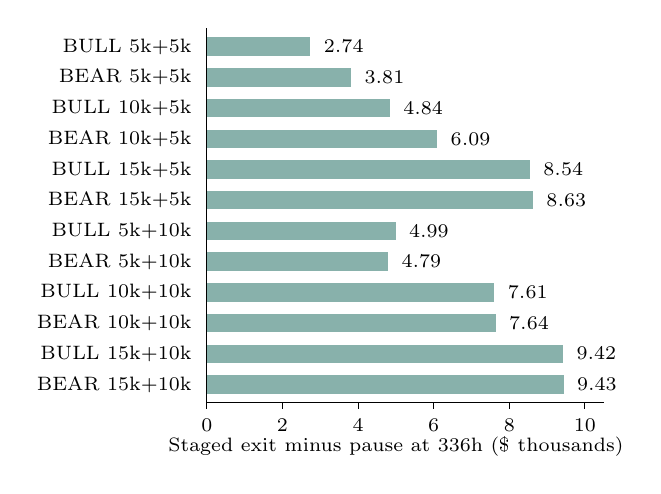
\begin{tikzpicture}[x=0.48cm,y=0.39cm,font=\scriptsize]
\foreach \lab/\val [count=\i] in {
 BULL 5k+5k/2.73637,
 BEAR 5k+5k/3.81432,
 BULL 10k+5k/4.83896,
 BEAR 10k+5k/6.09226,
 BULL 15k+5k/8.54469,
 BEAR 15k+5k/8.62541,
 BULL 5k+10k/4.99001,
 BEAR 5k+10k/4.79270,
 BULL 10k+10k/7.60652,
 BEAR 10k+10k/7.63833,
 BULL 15k+10k/9.42026,
 BEAR 15k+10k/9.43499}{
 \fill[teal!55] (0,-\i+0.3) rectangle (\val,-\i-0.3);
 \node[anchor=east] at (-0.15,-\i) {\lab};
 \node[anchor=west] at (\val+0.1,-\i) {\pgfmathprintnumber[fixed,precision=2]{\val}};
}
\draw (0,-0.4)--(0,-12.6)--(10.5,-12.6);
\foreach \v in {0,2,4,6,8,10} {\draw (\v,-12.6)--(\v,-12.8) node[below] {\v};}
\node[below] at (5,-13.4) {Staged exit minus pause at 336h (\$ thousands)};
\end{tikzpicture}
\caption{\rev{Cash difference $D_p$ for all 12 local \textit{Laya} plan pairs
at the common terminal hour 336. Labels give regime, founder position budget,
and upfront cost, in thousands of dollars. Unsold inventory is excluded;
therefore these bars do not rank total wealth.}}
\label{fig:matched-laya}
\end{figure}

\begin{revised}
Beyond coverage, the completed matrix exposes limits of the actor model.
\textit{Laya} produced similar traded cash across the two regimes:
\$8{,}493{,}778 in \textit{BULL} and \$8{,}282{,}843 in \textit{BEAR}, a gap
of approximately 2.5\%. Across 136{,}841 multi-option requests, its mean top
score was 0.42. Near-uniform option scores, combined with the engine's sampling
rule, are consistent with heavy two-way turnover and weak regime separation.
The recorded rejection count is about 1.30 per decision point. These
observations motivate behavioral validation rather than a market forecast.

Despite weak regime separation, staged exit held between \$2{,}736.37 and
\$9{,}434.99 more realized cash than pause in all 12 pairs at hour 336
(Figure~\ref{fig:matched-laya}). Founder purchases and exit tranches follow
explicit policy rules, so this cash comparison is not evidence that the actor
model discovered a superior strategy. In all six \$10{,}000-upfront pairs,
upfront spending alone meets the \$10{,}000 loss-budget alert at launch.

Including unsold inventory changes the interpretation. At hour 336 its pool
quote is between \$4{,}278 and \$11{,}805 under pause. Adding that quote to cash
puts pause ahead by \$464--\$3{,}260 in the six \$5{,}000-upfront pairs; staged
exit remains \$256--\$843 ahead in the six \$10{,}000-upfront pairs. A pool
quote is not guaranteed executable proceeds. The comparison must therefore
show realized cash and retained inventory separately.
\end{revised}

\subsection{NEAR Lending Case Study (RQ6)}\label{sec:res-lending}
\begin{revised}
Apart from sampled token trading, four local \textit{Laya} lending worlds
complete 90 days each (2{,}160 hours), with decisions selected by argmax.
Their event journals support exact ledger replay. Table~\ref{tab:lending}
summarizes only those four worlds; hosted and mixed-model runs are excluded.
\end{revised}

\begin{table}[t]
\caption{Local \textit{Laya} lending worlds after 90 days. Protocol share is 15\% of borrower
interest, collected plus still owed. Campaign spending was \$20{,}000 in each local world. ``Borrowed'' counts decisions in which borrowing was offered
and chosen.}
\label{tab:lending}
\centering\footnotesize\color{revisedred}
\renewcommand{\arraystretch}{1.1}\setlength{\tabcolsep}{3pt}
\begin{tabular}{@{}lrrrrr@{}}
\toprule
World & Lent, day 30 & Peak use & Liquid. & Protocol \$ & Borrowed \\
\midrule
C-P50-R2-L & \$300K & 15.6\% & 1 & 361 & 54/54 \\
C-P100-R2-L & \$500K & 25.8\% & 12 & 703 & 292/295 \\
C-P100-R8-L & \$500K & 25.8\% & 13 & 1{,}802 & 258/260 \\
B-P100-R8-L & \$374K & 19.5\% & 20 & 1{,}077 & 431/433 \\
\bottomrule
\end{tabular}
\end{table}

First, the observed borrowing ceilings reflect explicit caps, while whether
actors reach them depends on their choices. In C-P50-R2-L each of the six borrowing
accounts reached its \$50{,}000 cap by day 30, and once that cap was raised,
both \textit{Laya} choppy worlds reached the \$500{,}000 aggregate cap by the
same day. With about \$2{,}000{,}000 supplied, utilization could not exceed
about 25\%. Under Eq.~\eqref{eq:rate}, suppliers therefore earned about 1\% a
year under curve R2 and 2.4\% under R8, against \textit{RHEA}'s 9.88\%;
matching \textit{RHEA} at 25\% utilization would require a borrow rate near
46\%. Second, the risk rules left no bad debt in any world, and the loss
reserve was never used. On the bear path, hourly closes fell 68\% and twenty
liquidations repaid \$302{,}000 without loss.

That second result carries two conditions. It depends on the assumed
liquidators' cash and exit depth, which were not measured, and on the
oracle's hourly sampling. On 10 October 2025 NEAR briefly traded 40\% below
the choppy window's opening price but closed that hour about 9\% lower, so the
deepest fall the ledger saw on that path was 31\%, and its liquidations came
on days 60--61, 67, and 80--85. Liquidations during such intrahour moves remain
untested.

\begin{revised}
The behavioral observations require a different interpretation.
Borrowing was selected in 258 of 260 offered decisions under curve R8 and
292 of 295 under curve R2 in the choppy worlds. This near-saturation persists
despite materially different rates and should not be read as measured demand.
Partner acceptance, supply retention, and campaign reach also depend on
uncalibrated model choices and synthetic balances. Real borrower intentions,
observed conversion, and multiple seeds are needed before extrapolating those
behaviors.
\end{revised}

Within these four worlds, the launch's modeled economics are thin. Over 90 days, the
protocol's share of interest ranged from \$361 to \$1{,}802 in the
\textit{Laya} worlds, against \$20{,}000 spent on the campaign.

\section{Discussion and Limitations}\label{sec:discussion}
The results in Section~\ref{sec:results} establish what the system does
reliably and where its evidence stops. This section interprets them, explains
the local actor-inference boundary, relates \textit{Boyun} to
\textit{MiroFish}, and sets out the work needed before any predictive claim
could be made.

\subsection{What the Results Show}
\begin{revised}
Taken together, the mechanism checks answer RQ1 and RQ2 within their stated
scope: arithmetic, timing, accounting, and saved-decision replay agree with
specified rules. Changing individual mechanisms changes results in controlled
ways. In particular, the offline preference test demonstrates that changing
numeric weights affects its policy, whereas rewriting persona prose alone does
not. That test does not establish how a learned actor model interprets either.

Extending those checks to a larger setting, local \textit{Laya} inference
carries all 24 token-launch paths through 336 hours. This verifies the ability
to record and settle repeated actor decisions without a per-call API fee.
It does not validate the regime hypotheses or the trading behavior. Realized
cash favors staged exit in the observed pairs, yet including inventory quotes
changes that comparison in six pairs. The metric selected therefore affects
what a reader may conclude.

Apart from trading, the four local lending worlds distinguish a numerical
constraint from behavior that happens to reach it. A borrower cap limits the
maximum possible loan, but reaching that cap depends on model choices. Likewise,
zero observed bad debt is conditional on the tested prices, liquidation rules,
liquidator resources, and depth. Reports should identify these assumptions
rather than treating either result as an unconditional property of a launch.
\end{revised}

\subsection{Self-Hosted Actor Inference}
\begin{revised}
The local execution path addresses a practical privacy requirement:
world observations can be scored on the user's hardware instead of being sent
to a hosted actor API. This narrows a data-transfer boundary; it is not a proof
of system-wide confidentiality. External data services, optional commitments,
artifact sharing, and host access remain separate considerations. Zero API
fee likewise excludes hardware, electricity, setup, and maintenance costs.

Within that local path, \textit{Laya}'s limitations are consequential.
Its context is limited to 1024 tokens, observations that would be truncated are
rejected, and its option scores are uncalibrated \cite{layamodel}. The recorded
trading distributions show limited regime separation, while lending choices
frequently select borrowing under both tested rate curves. These patterns
should motivate validation against actual behavior, not be presented as
measured investor or borrower demand.

Looking beyond the current experiments, other open-weight typed models, such
as \textit{Kev}, are candidates for comparison \cite{kevrepo}. They have not
been evaluated in these case studies, and compatibility alone would not imply
behavioral quality. Multiple seeds, measured demand, and matched evaluations
are stronger next steps than claiming predictive value from local inference
or from agreement between models.
\end{revised}

\subsection{Relation to \textit{MiroFish}}
The comparison with \textit{MiroFish} suggests a division of labor rather than
a contest. \textit{MiroFish} produces rich, persona-specific discourse but no
financial consequences; \textit{Boyun} produces settled, replayable financial
consequences but only pre-written messages. A natural next step is to let
language-model actors write \textit{Boyun}'s messages while the engine keeps
control of delivery, timing, and settlement, so that what an actor says
is generated freely but what it can see and spend is still enforced. Doing so
would raise the cost per decision and introduce new questions about how text
should influence trading, which would need their own evaluation.

\subsection{Toward Predictive Validation}
None of the tests in this paper measures forecasting accuracy, and
Figure~\ref{fig:validation} outlines what such a test would require. A study
must first fix one measurable outcome, its resolution source, and its
horizon, and freeze the world-construction procedure, models, and evidence
cutoff before any forecast is issued. Forecasts must then be dated and kept,
including failed runs, and scored against resolved outcomes using
Eqs.~\eqref{eq:brier} and~\eqref{eq:logloss}, alongside simple baselines such
as a historical base rate and a single-model forecast given the same
evidence. Cases that share a time period or narrative are not independent and
must be treated as such when estimating uncertainty. A separate user study
would be needed to test whether \textit{Boyun}'s reports improve decisions,
which is a different question from whether its probabilities are accurate.

\begin{figure}[t]
\centering
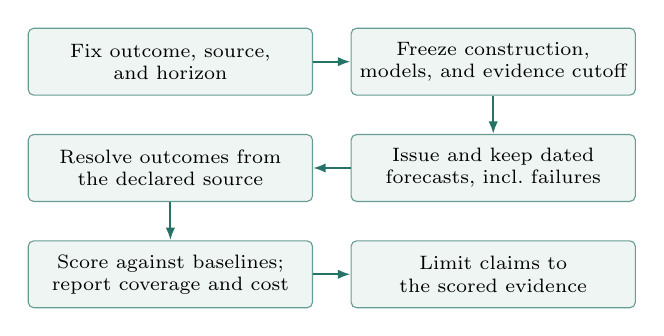
\begin{tikzpicture}[font=\scriptsize,
 vstep/.style={draw=teal!70,fill=wash,rounded corners=2pt,align=center,text width=3.4cm,minimum height=0.85cm,inner sep=3pt},
 arr/.style={-{Latex[length=1.6mm]},thick,draw=teal}]
\node[vstep] (a) at (0,0) {Fix outcome, source,\\and horizon};
\node[vstep] (b) at (4.1,0) {Freeze construction,\\models, and evidence cutoff};
\node[vstep] (c) at (4.1,-1.35) {Issue and keep dated\\forecasts, incl.\ failures};
\node[vstep] (d) at (0,-1.35) {Resolve outcomes from\\the declared source};
\node[vstep] (e) at (0,-2.7) {Score against baselines;\\report coverage and cost};
\node[vstep] (f) at (4.1,-2.7) {Limit claims to\\the scored evidence};
\draw[arr] (a)--(b); \draw[arr] (b)--(c); \draw[arr] (c)--(d);
\draw[arr] (d)--(e); \draw[arr] (e)--(f);
\end{tikzpicture}
\caption{Proposed prospective validation protocol. This is future work,
not an experiment reported in this paper.}
\label{fig:validation}
\end{figure}

\subsection{Limitations}
\begin{revised}
Several limitations apply to the full evaluation. The case results use one
seed per plan, synthetic actor balances and preferences, and declared event or
price schedules. They do not represent independent observations of human
behavior. In \textit{MACRON}, near-uniform option scores weaken regime
separation, and upfront spending alone triggers the loss-budget alert in the
higher-upfront plans. Founder trades are partly policy-driven, so model choice
cannot explain every cash difference.

On the market side, a simplified constant-product pool omits order books,
transaction ordering, front-running, outages, and venue-specific execution
details. On the lending side, assumed liquidator cash and exit depth determine
which liquidations can settle; historical hourly closes do not test intrahour
price shocks. The competing venue's rates are fixed at one snapshot and campaign
reach has no measured conversion. These conditions bound the scope of every
financial conclusion.

Finally, messages attached to actions are pre-written, giving \textit{Boyun}
a narrower social layer than open-ended discourse. The \textit{MiroFish}
comparison matches the brief, but actor models, activation rules, and recovery
procedures differ. It compares recorded capabilities rather than forecasting
accuracy or general superiority.
\end{revised}

\subsection{Responsible Use}
These limits also shape how \textit{Boyun} should and should not be used.
Its outputs are conditional explorations of stated assumptions, not
financial advice or price forecasts. Because the case study concerns paid
promotion of a speculative token, the same tools could in principle be used to
rehearse campaigns that mislead buyers; reports therefore state their
assumptions and limits explicitly, and they should not be presented to
investors as evidence of likely returns. World files and reports can contain
private strategy, so authors should share them deliberately. Local actor
inference avoids sending observations to an actor API; external services and
publication remain separate disclosure decisions.

\section{Conclusion}\label{sec:conclusion}
\begin{revised}
This paper examined how an explicitly specified multi-agent world constrains
actor observations, actions, and settlement while preserving records of the
resulting choices and consequences. \textit{Boyun} combines game-theoretic
specification, directed information graphs, typed local actor inference, and
ledger-specific execution. Saved decisions support deterministic replay,
while model scores remain distinct from calibrated event probabilities.

Within this design, synthetic checks verify calculations and isolate selected
mechanisms. A full-horizon local \textit{Laya} token-launch matrix records
24 paths through fourteen days, while four local lending worlds cover ninety
days each. The same-brief comparison with \textit{MiroFish} illustrates the
difference between generating social discourse and settling financial actions;
it does not establish a performance ranking. Case outcomes remain conditional
on their policies, synthetic actors, and execution assumptions.

The next steps follow from these evidence boundaries: test multiple seeds and
alternative open-weight models, measure behavior rather than assume demand,
and evaluate dated forecasts against resolved outcomes. Self-hosted inference
provides a useful execution option, but the quality of the resulting financial
analysis must be established separately.
\end{revised}

\bibliographystyle{IEEEtran}
\bibliography{references}
\end{document}
